% \iffalse
%<*driver>
\documentclass{ltxdoc}
\usepackage[UTF8]{ctex}
\usepackage{geometry}
\usepackage{hyperref}
\usepackage{xcolor}
\usepackage{hologo}% 与手册正文中 \hologo{XeLaTeX} 等徽标一致
% 说明文档使用 \DescribeMacro/\DescribeEnv 时在左侧旁注排版名称；
% 对称 margin=2.5cm 时常使 marginpar 过窄，长环境名（如 acknowledgements）会挤在一起。
\geometry{%
  a4paper,
  left=3.8cm,
  right=2.5cm,
  top=2.5cm,
  bottom=2.5cm,
  marginparwidth=3.2cm,
  marginparsep=6pt}
% doc 中 theindex / theglossary 使用 multicols；若当前页底部剩余高度过小，
% 仍会开始 multicols 从而在输出例程中报 “Error saving partial page”。
% 增大 \IndexMin / \GlossaryMin 可在版面过满时先换页（见 multicol 与 doc 说明）。
\AtBeginDocument{%
  \setlength{\IndexMin}{15\baselineskip}%
  \setlength{\GlossaryMin}{15\baselineskip}}
% doc 默认三栏索引；栏宽过窄时，长控制序列名在 \texttt 中易 Overfull。
\setcounter{IndexColumns}{2}
\EnableCrossrefs
\CodelineIndex
\RecordChanges
\begin{document}
\DocInput{swuthesis.dtx}
\end{document}
%</driver>
% \fi
%
% \GetFileInfo{swuthesis.dtx}
%
% \title{\textsf{swuthesis}: 西南大学博士后/博士/硕士/本科毕业论文模板}
% \author{Van Abel}
% \date{\today}
%
% \maketitle
%
% \begin{abstract}
% 本文件为 \textsf{swuthesis} 的 \texttt{.dtx} 文档源码，
% 用于统一管理代码实现与文档说明。其目标是支持：
% \begin{itemize}
%   \item 模板选项说明；
%   \item 用户命令说明；
%   \item 用户环境说明；
%   \item 完整的使用文档。
% \end{itemize}
% \end{abstract}
%
% \tableofcontents
%
% \section{简介}
%
% \textsf{swuthesis} 用于生成西南大学博士后、博士、硕士、本科毕业论文。
% 推荐采用 \texttt{dtx+ins} 方式维护：
% \begin{itemize}
%   \item 代码与说明写在同一个 \texttt{.dtx} 文件中；
%   \item 通过 \texttt{docstrip} 抽取出 \texttt{.cls}/\texttt{.sty} 文件；
%   \item 通过 \texttt{ltxdoc} 直接生成用户手册。
% \end{itemize}
%
% \section{安装与生成}
%
% 目录中至少包含以下文件：
% \begin{quote}
% \texttt{swuthesis.dtx}\par
% \texttt{swuthesis.ins}
% \end{quote}
%
% 其中：
% \begin{itemize}
%   \item \texttt{swuthesis.dtx} 同时维护类文件代码、示例文档和用户手册；
%   \item \texttt{swuthesis.ins} 负责用 \texttt{docstrip} 抽取
%         \texttt{swuthesis.cls} 与 \texttt{swuthesis.tex}；
%   \item \texttt{Makefile} 负责统一封装构建命令。
% \end{itemize}
%
% 推荐的工作流如下：
% \begin{verbatim}
% latex swuthesis.ins
% xelatex swuthesis.tex
% xelatex swuthesis.dtx
% makeindex -s gind.ist swuthesis.idx
% makeindex -s gglo.ist -o swuthesis.gls swuthesis.glo
% xelatex swuthesis.dtx
% \end{verbatim}
% 第一步会生成 \texttt{swuthesis.cls}、\texttt{swuthesis-main.tex}（本科示例）与
% \texttt{swuthesis-doctor-main.tex}（博士示例）；
% 第二步用于验证模板示例；后续步骤用于生成说明文档。
% 由于文档中包含中文并依赖 \texttt{ctex}，示例文档和说明文档都应使用
% \hologo{XeLaTeX} 编译。
%
% \section{用户接口概览}
%
% \subsection{模板选项}
%
% 模板支持如下主要选项：
% \begin{description}
%   \item[postdoc] 博士后报告模式。
%   \item[doctor] 博士论文模式。
%   \item[master] 硕士论文模式。
%   \item[bachelor] 本科论文模式。
%   \item[print] 打印版模式。
%   \item[oneside] 单面排版（默认，可省略不写）。
%   \item[twoside] 双面排版（传给 \texttt{book}，覆盖默认的 \texttt{oneside}）。
% \end{description}
%
% \paragraph{博士/硕士与《西南大学博士、学术型硕士学位论文规范》}
% 选用 |doctor| 或 |master| 时，模板会按该规范倾向调整：版芯与学校要求一致；
% 章/节/条标题分别为黑体三号、四号、小四号；正文小四号宋体、行距约 20 磅；
% 图/表题五号黑体；参考文献表为顺序编码制（|biblatex| 样式 |gb7714-2025|，与本科一致），
% |\cite| 为角标；自摘要页起页眉为「西南大学博士/硕士学位论文」与各章章名，
% 页眉下为文武线；目录一般列至二级标题。书脊、双面页码位置等印刷细节请在定稿后按当年研究生院通知处理。
%
% \DescribeMacro{\swusetup}
% 用于集中设置论文元信息（不含中英文摘要与关键词；后者使用 |cnabstract|、|cnkeywords|、|enabstract|、|enkeywords| 环境）。
% \begin{verbatim}
% \swusetup{
%   title        = {论文题目},
%   author       = {作者姓名},
%   student-id   = {学号},
%   supervisor   = {指导教师},
%   degree       = {硕士},
%   major        = {基础数学},
%   research-field = {研究方向（博士模板可选）},
%   degree-en    = {the degree of Doctor of Philosophy in Mathematics},
%   supervisor-en = {Prof.\ Jane Doe},
%   graduate-program-en = {Graduate Program in Department of Mathematics},
%   submitted-school-en = {Graduate School},
%   university-en = {Southwest University},
%   defense-location-en = {Chongqing, P.R. China},
%   submit-year = {2026},
%   submit-month = {3},
%   submit-day = {15}
% }
% 博士中文封面信息区含：论文作者、指导教师、学科专业、研究方向、提交日期、答辩日期、授予单位（西南大学）；
% 页脚为「中国重庆」与答辩年月。|submit-*| 为空时提交日期仅显示下划线。
% 博士英文题名页为单页：|title-en|/|author-en| 大写；|degree-en| 填在「For the degree of」下一行；「And approved by」下为
% 五条签名横线。|submitted-school-en|、|university-en|、|defense-location-en| 留空时分别为 |Graduate School|、
% |Southwest University|、|Chongqing, P.R. China|（西南大学）；页底为英文月份 + |defense-year|。若外方联合培养需仿
% Rutgers 地名，可自行设 |defense-location-en|。
% \end{verbatim}
%
% \subsection{用户命令}
%
% \DescribeMacro{\maketitlepage}
% 生成论文封面与题名页（含本科独创声明等）。
% 本科与博士中文封面均使用目录 |figures/| 下的 |swu-badge.pdf|（校徽）、|swu-name-stxingkai.pdf|（华文行楷横排校名）；
% 若另有 |swu-name.pdf|（常见为英文或通用横排校名），置于同目录时由类文件自动排于行楷校名之下；无该文件亦可编译。
%
% \DescribeMacro{\maketitle}
% 与 \LaTeX{} 习惯一致，定义为 |\maketitlepage| 的别名；并非 \texttt{article} 类中基于
% |\title|/|\author|/|\date| 的简易标题页，论文元信息仍由 |\swusetup| 提供。
%
% \DescribeMacro{\makeabstract}
% 根据 |cnabstract|、|cnkeywords|、|enabstract|、|enkeywords| 环境已写入的内容，生成中英文摘要版面（须先写上述环境，再调用本命令）。
%
% \DescribeMacro{\makegraduateoriginalitystatement}
% 生成独创性声明与学位论文版权使用授权书（合排一页；题目行仿宋、行末横线拉至版心右端，多行时请在 |title| 中用 |\\| 断行）。
% 在 |doctor| 模式下由 |\maketitlepage| 内部调用，一般无需在文档中手动书写。
%
% \DescribeEnv{cnabstract}
% \DescribeEnv{cnkeywords}
% \DescribeEnv{enabstract}
% \DescribeEnv{enkeywords}
% 分别收录中文摘要正文、中文关键词、英文摘要正文、英文关键词；内容写在 |\begin{document}| 之后、|\makeabstract| 之前。
%
% \subsection{用户环境}
%
% \DescribeEnv{acknowledgements}
% 致谢环境：标题「致谢」为居中、小四号加粗宋体；正文为五号宋体、单倍行距，段首缩进两格（与正文一致）；
% 正文段前、段后各约半行：标题与首段之间、末段之后各插入半行垂直间距；段与段之间段距取一行高
% （相当于相邻两段在规范中各设半行段前、段后时之净距）。
%
% \DescribeEnv{resume}
% 作者简介环境。
%
% \DescribeEnv{publications}
% |在读期间取得的科研成果|：版式与 |acknowledgements| 相近（居中标题、五号宋体、目录收录），
% 宜置于致谢之后、附录之前。条目中可用 |\swupublicationsubsection| 划分
% 「已发表论文」「发明专利」「会议论文」「参与的科研项目」等，并用 |swupubenum| 环境
% 产生 |[1]|、|[2]| 形式编号（各小节内独立编号）。
%
% \DescribeMacro{\swupublicationsubsection}
% |\swupublicationsubsection{小标题}|：在 |publications| 环境内插入一条加粗小标题
% （如「已发表论文：」），与下列表项之间的垂直间距已略调。
%
% \DescribeEnv{swupubenum}
% 编号列表环境，|enumerate| 的 |label| 为 |[1]|、|[2]|、\ldots，便于科研成果分条列举。
%
% \DescribeEnv{theorem}
% \DescribeEnv{lemma}
% \DescribeEnv{proposition}
% \DescribeEnv{corollary}
% \DescribeEnv{hypothesis}
% \DescribeEnv{definition}
% \DescribeEnv{example}
% \DescribeEnv{remark}
% \DescribeEnv{thm}
% \DescribeEnv{lem}
% \DescribeEnv{prop}
% \DescribeEnv{cor}
% \DescribeEnv{hyp}
% \DescribeEnv{defn}
% \DescribeEnv{ex}
% \DescribeEnv{rmk}
% 正文中的定理类环境由 \textsf{amsthm} 提供，按章编号并与式、图、表等共享递增序列。
% 版式按常见中文规范：定理、定义、引理等\textbf{顶格}（相对版心左对齐起排），编号与正文之间
% 空约一格宽；正文段落首行缩进两格，定理内若分段，自第二段起与正文相同缩进。
% 标题为加粗宋体，正文为楷体（与正文同字号）；\verb|proof| 环境标题行仍为加粗宋体，
% 证明正文为宋体小四，与正文默认一致。
% 同时提供缩写环境名（如 \verb|thm|、\verb|lem|、\verb|hyp|、\verb|defn|、\verb|rmk| 等），与全称环境共享计数器与标题，
% 可任选其一书写；其中定义不用 \verb|def|（与 \TeX{} 的 \verb|\def| 冲突），缩写为 \verb|defn|。
% 交叉引用推荐使用 \textsf{cleveref} 的 \verb|\cref|/\verb|\Cref|，例如
% \verb|\cref{thm:main}|（标签前缀习惯用 \texttt{thm:} 等，与环境名无关）。
% 多标签并列时连接词已设为中文：两项之间为「和」，三项及以上中间为顿号、最后一项前为「与」；范围用「至」。
%
% \section{基本使用示例}
%
% \begin{verbatim}
% \documentclass[master,twoside]{swuthesis}
%
% \swusetup{
%   title      = {西南大学学位论文模板设计},
%   author     = {张三},
%   supervisor = {李四教授},
%   major      = {基础数学},
%   degree     = {理学硕士}
% }
%
% \begin{document}
% \frontmatter
% \maketitle
% \tableofcontents
% \begin{cnabstract}
% 中文摘要\ldots
% \end{cnabstract}
% \begin{cnkeywords}
% 关键词一；关键词二
% \end{cnkeywords}
% \begin{enabstract}
% English abstract\ldots
% \end{enabstract}
% \begin{enkeywords}
% keyword one; keyword two
% \end{enkeywords}
% \makeabstract
% \mainmatter
% \chapter{引言}
% 正文内容。
% \backmatter
% \begin{acknowledgements}
% 感谢……
% \end{acknowledgements}
% \end{document}
% \end{verbatim}
%
% 上述示例也可以直接由 \texttt{swuthesis.dtx} 抽取为
% \texttt{swuthesis-main.tex}，便于测试类文件是否可正常使用。
%
% \StopEventually{\PrintChanges\PrintIndex}
%
% \section{实现说明}
%
% \subsection{类文件声明}
%
%    \begin{macrocode}
%<*class>
\NeedsTeXFormat{LaTeX2e}
\ProvidesClass{swuthesis}[2026/04/17 v0.1 Southwest University thesis template]
\RequirePackage{kvoptions}
\SetupKeyvalOptions{family=swu,prefix=swu@}
\DeclareBoolOption[false]{postdoc}
\DeclareBoolOption[false]{doctor}
\DeclareBoolOption[false]{master}
\DeclareBoolOption[false]{bachelor}
\DeclareBoolOption[false]{print}
\newif\ifswu@twoside
\swu@twosidefalse
\DeclareVoidOption{oneside}{\swu@twosidefalse}
\DeclareVoidOption{twoside}{\swu@twosidetrue}
\ProcessKeyvalOptions*
\ifswu@twoside
  \LoadClass[12pt,a4paper,twoside]{book}
\else
  \LoadClass[12pt,a4paper,oneside]{book}
\fi
% 《西南大学博士、学术型硕士学位论文规范》：博士/硕士共用版式与页眉等；参考文献默认与本科同为顺序编码制。
\newif\ifswu@gradthesis
\swu@gradthesisfalse
\ifswu@doctor
  \swu@gradthesistrue
\else\ifswu@master
  \swu@gradthesistrue
\fi\fi
\makeatletter
%
\RequirePackage{xparse}
\RequirePackage{etoolbox}
\RequirePackage[heading=true,zihao=-4]{ctex}
\setmainfont{Times New Roman}
\RequirePackage{amsmath,amssymb}
\RequirePackage{amsthm}
\RequirePackage{aliascnt}
\RequirePackage{geometry}
\RequirePackage{setspace}
\RequirePackage{enumitem}
\RequirePackage{fancyhdr}
\RequirePackage[bookmarksnumbered=true]{hyperref}
\RequirePackage{bookmark}
\RequirePackage{hologo}% \hologo{XeLaTeX} 等引擎与格式名称的专业排版
\RequirePackage{xurl}
\RequirePackage{graphicx}
\RequirePackage{xcolor}
\RequirePackage{tocloft}
\RequirePackage{caption}
\RequirePackage{booktabs}
\RequirePackage{array}
\RequirePackage{listings}
% 各学位统一：|gb7714-2025| 顺序编码制（|sorting=none|，文后表按引用先后编号）。
% 若须著者-出版年制，可改为 |style=gb7714-2025ay| 并去掉下文 |\let\cite\supercite|。
\RequirePackage[
  backend=biber,
  style=gb7714-2025,
  sorting=none,
  doi=false,
  url=false,
  eprint=true
]{biblatex}
\DeclareFieldFormat{eprint:arxiv}{%
  \mkbibacro{arXiv}\addcolon\space\href{https://arxiv.org/abs/#1}{#1}%
  \iffieldundef{eprintclass}{}{\space\mkbibbrackets{\thefield{eprintclass}}}%
}
% biber 可能将 arXiv 的 eprinttype 规范为 |arxiv| 或保留 |arXiv|，二者皆视为 arXiv 预印本，避免重复输出网址
\AtEveryBibitem{%
  \ifboolexpr{ test {\iffieldequalstr{eprinttype}{arxiv}} or test {\iffieldequalstr{eprinttype}{arXiv}} }%
    {%
      \clearfield{url}%
      \clearfield{urlraw}%
      \clearfield{urldate}%
      \clearlist{institution}%
    }{}%
}
\renewbibmacro*{modifydate}{%
  \ifboolexpr{ test {\iffieldequalstr{eprinttype}{arxiv}} or test {\iffieldequalstr{eprinttype}{arXiv}} }%
    {\usebibmacro{newsdate}}
    {%
      \iffieldundef{eventday}%
         {%
           \iffieldundef{endday}{%
               \iffieldundef{day}{%
               \iffieldundef{year}{}
                 {\printtext{\gbleftparen}\blx@gbdate{}{}\printtext{\gbrightparen}}%
               }%
               {\printtext{\gbleftparen}\blx@gbdate{}{}\printtext{\gbrightparen}}%
               }%
              {\printtext{\gbleftparen}\printenddate\printtext{\gbrightparen}}%
         }%
         {\printtext{\gbleftparen}\printeventdate\printtext{\gbrightparen}}%
    }%
}
% 电子资源引用日期：|biblatex-gb7714| 默认仅输出 |[日期]|，此处标明为访问日期：
\renewbibmacro*{urldate}{%
  \addthinspace
  \printtext{访问日期}%
  \printtext{：}\printurldate%
}
% 顺序编码制下将 |\cite| 定为角标（与学校常见「上标序号」一致）。
\let\cite\supercite
%
% 定理类环境（\textsf{amsthm}）：各环境借助 \textsf{aliascnt} 拥有独立计数器名称，
% 以便 \textsf{cleveref} 的 \verb|\cref| 正确区分引理、命题等（编号仍随章内定理序列递增）。
% 版式：标题加粗宋体，正文楷体（与正文同字号小四）。
% \textsf{amsthm} 第 5 个参数为「标题前缩进量」：误用 \cs{parindent} 会在标题前插入空盒，
% 导致整块定理右移；留空则为顶格，与中文习惯「定理等顶格、正文段落首行缩进」一致。
% 第 8 个参数为标题与正文间距，取 |1\ccwd| 表示编号后空一格再接内容。
% 定理内分段时，自第二段起沿用全文 \cs{parindent}（请在导言区或 \cs{mainmatter} 中设定
% 正文首行缩进，如 |\setlength{\parindent}{2\ccwd}|）。
\newtheoremstyle{swuplain}%
  {3pt}{3pt}%
  {\normalfont\kaishu\zihao{-4}}%
  {}%
  {\normalfont\songti\bfseries\zihao{-4}}%
  {.}{1\ccwd}%
  {}
\newtheoremstyle{swudefinition}%
  {3pt}{3pt}%
  {\normalfont\kaishu\zihao{-4}}%
  {}%
  {\normalfont\songti\bfseries\zihao{-4}}%
  {.}{1\ccwd}%
  {}
\newtheoremstyle{swuremark}%
  {3pt}{3pt}%
  {\normalfont\kaishu\zihao{-4}}%
  {}%
  {\normalfont\songti\bfseries\zihao{-4}}%
  {.}{1\ccwd}%
  {}
\theoremstyle{swuplain}
\newtheorem{theorem}{定理}[chapter]
\newaliascnt{lemma}{theorem}
\newtheorem{lemma}[lemma]{引理}
\aliascntresetthe{lemma}
\newaliascnt{proposition}{theorem}
\newtheorem{proposition}[proposition]{命题}
\aliascntresetthe{proposition}
\newaliascnt{corollary}{theorem}
\newtheorem{corollary}[corollary]{推论}
\aliascntresetthe{corollary}
\newaliascnt{hypothesis}{theorem}
\newtheorem{hypothesis}[hypothesis]{假设}
\aliascntresetthe{hypothesis}
\theoremstyle{swudefinition}
\newaliascnt{definition}{theorem}
\newtheorem{definition}[definition]{定义}
\aliascntresetthe{definition}
\newaliascnt{example}{theorem}
\newtheorem{example}[example]{例}
\aliascntresetthe{example}
\theoremstyle{swuremark}
\newaliascnt{remark}{theorem}
\newtheorem{remark}[remark]{注}
\aliascntresetthe{remark}
% 缩写环境（与上列全称共享计数器；标题与 \cref 类型名与全称一致）
\newtheorem{thm}[theorem]{定理}
\newtheorem{lem}[lemma]{引理}
\newtheorem{prop}[proposition]{命题}
\newtheorem{cor}[corollary]{推论}
\newtheorem{hyp}[hypothesis]{假设}
\newtheorem{defn}[definition]{定义}
\newtheorem{ex}[example]{例}
\newtheorem{rmk}[remark]{注}
% 证明环境：标题行加粗宋体；正文宋体小四（与 \cs{swumainmatterstyle} 正文一致，非定理楷体）
\renewenvironment{proof}[1][\proofname]{%
  \par\pushQED{\qed}%
  \normalfont\topsep6\p@\@plus6\p@\relax
  \trivlist
  \item[\hskip\labelsep\normalfont\songti\bfseries\zihao{-4}#1\@addpunct{.}]%
  \ignorespaces\normalfont\songti\zihao{-4}%
}{%
  \popQED\endtrivlist\@endpefalse
}%
\RequirePackage[nameinlink]{cleveref}
\crefname{theorem}{定理}{定理}
\Crefname{theorem}{定理}{定理}
\crefname{lemma}{引理}{引理}
\Crefname{lemma}{引理}{引理}
\crefname{proposition}{命题}{命题}
\Crefname{proposition}{命题}{命题}
\crefname{corollary}{推论}{推论}
\Crefname{corollary}{推论}{推论}
\crefname{hypothesis}{假设}{假设}
\Crefname{hypothesis}{假设}{假设}
\crefname{definition}{定义}{定义}
\Crefname{definition}{定义}{定义}
\crefname{example}{例}{例}
\Crefname{example}{例}{例}
\crefname{remark}{注}{注}
\Crefname{remark}{注}{注}
\crefname{equation}{式}{式}
\Crefname{equation}{式}{式}
\crefname{figure}{图}{图}
\Crefname{figure}{图}{图}
\crefname{table}{表}{表}
\Crefname{table}{表}{表}
% cleveref 多引用时的连接词（默认英文 |and|）；在 |\begin{document}| 后再设，以免被语言定义覆盖。
\AtBeginDocument{%
  \renewcommand{\crefpairconjunction}{ 和 }%
  \renewcommand{\crefmiddleconjunction}{、}%
  \renewcommand{\creflastconjunction}{ 与 }%
  \renewcommand{\crefpairgroupconjunction}{ 和 }%
  \renewcommand{\crefmiddlegroupconjunction}{、}%
  \renewcommand{\creflastgroupconjunction}{ 与 }%
  \renewcommand{\crefrangeconjunction}{至\nobreakspace}%
  % 「第…章/节」须用 \creflabelformat：|nameinlink| 只在标签层给编号加链接；
  % 若用 \crefformat 把「第」「章」写在外层，则超链接仅覆盖编号。
  % 类型名置空，避免与「第…章」重复；附录中的 |\chapter| 仍勿用 |\cref|。
  \crefname{chapter}{}{}%
  \Crefname{chapter}{}{}%
  \creflabelformat{chapter}{第#2#1#3章}%
  \crefrangelabelformat{chapter}{第#3#1#4章至第#5#2#6章}%
  \crefname{section}{}{}%
  \Crefname{section}{}{}%
  \creflabelformat{section}{第#2#1#3节}%
  \crefrangelabelformat{section}{第#3#1#4节至第#5#2#6节}%
  \crefname{subsection}{}{}%
  \Crefname{subsection}{}{}%
  \creflabelformat{subsection}{第#2#1#3小节}%
  \crefrangelabelformat{subsection}{第#3#1#4小节至第#5#2#6小节}%
  \crefname{subsubsection}{}{}%
  \Crefname{subsubsection}{}{}%
  \creflabelformat{subsubsection}{第#2#1#3目}%
  \crefrangelabelformat{subsubsection}{第#3#1#4目至第#5#2#6目}%
  \hypersetup{pdflang=zh-CN}%
  \def\chapterautorefname{章}%
  \def\sectionautorefname{节}%
  \def\subsectionautorefname{小节}%
  \def\subsubsectionautorefname{目}%
  \def\equationautorefname{式}%
  \def\figureautorefname{图}%
  \def\tableautorefname{表}%
  % cleveref 在 |\begin{document}| 之初已按当时定义生成 |\cref@…@format|；此后才执行的
  % |\creflabelformat| 不会自动重算外层引用格式，会导致 |\cref| 仅显示阿拉伯数字。
  \@crefdefineallformats{chapter}%
  \@crefdefineallformats{section}%
  \@crefdefineallformats{subsection}%
  \@crefdefineallformats{subsubsection}%
}
% 规范：图、表题用五号黑体（本科模板沿用原宋体五号）。
\ifswu@gradthesis
\DeclareCaptionFont{swucaptionfont}{\heiti\zihao{5}}
\else
\DeclareCaptionFont{swucaptionfont}{\songti\zihao{5}}
\fi
\captionsetup{
  font=swucaptionfont,
  labelfont=swucaptionfont
}
\lstdefinestyle{swucode}{
  backgroundcolor=\color{gray!8},
  basicstyle=\ttfamily\small,
  keywordstyle=\color{blue!70!black}\bfseries,
  commentstyle=\color{green!40!black},
  stringstyle=\color{orange!60!black},
  numbers=none,
  linewidth=\linewidth,
  xleftmargin=0pt,
  xrightmargin=0pt,
  columns=fullflexible,
  keepspaces=true,
  frame=single,
  rulecolor=\color{gray!40},
  frameround=tttt,
  breaklines=true,
  breakatwhitespace=false,
  breakindent=0pt,
  showstringspaces=false,
  tabsize=2
}
\lstdefinestyle{swucodeprint}{
  backgroundcolor=\color{white},
  basicstyle=\ttfamily\small,
  keywordstyle=\bfseries,
  commentstyle=\itshape,
  stringstyle=\ttfamily,
  numbers=none,
  linewidth=\linewidth,
  xleftmargin=0pt,
  xrightmargin=0pt,
  columns=fullflexible,
  keepspaces=true,
  frame=single,
  rulecolor=\color{black},
  frameround=tttt,
  breaklines=true,
  breakatwhitespace=false,
  breakindent=0pt,
  showstringspaces=false,
  tabsize=2
}
\renewcommand{\lstlistingname}{代码}
\renewcommand{\lstlistlistingname}{代码目录}
% 版芯：与学校本科规范及《西南大学博士、学术型硕士学位论文规范》一致（左/右 25mm，上 30mm，下 25mm，
% 装订线 10mm，页眉边距 23mm，页脚边距 18mm）；模板默认 |oneside|，双面时用 |twoside|。
\geometry{
  a4paper,
  left=25mm,
  right=25mm,
  top=30mm,
  bottom=25mm,
  bindingoffset=10mm,
  headsep=23mm,
  footskip=18mm
}
\ifswu@print
  \lstset{style=swucodeprint}
\else
  \lstset{style=swucode}
\fi
%
% 规范：目次一般只列到二级标题。
\ifswu@gradthesis
  \setcounter{tocdepth}{2}
\else
  \setcounter{tocdepth}{3}
\fi
\renewcommand{\cfttoctitlefont}{\hfill\heiti\zihao{3}}
\renewcommand{\cftaftertoctitle}{\hfill}
\setlength{\cftbeforetoctitleskip}{\baselineskip}
\setlength{\cftaftertoctitleskip}{2\baselineskip}
\renewcommand{\cftchapfont}{\songti\zihao{-4}}
\renewcommand{\cftsecfont}{\songti\zihao{-4}}
\renewcommand{\cftsubsecfont}{\songti\zihao{-4}}
\renewcommand{\cftchappagefont}{\rmfamily\zihao{-4}}
\renewcommand{\cftsecpagefont}{\rmfamily\zihao{-4}}
\renewcommand{\cftsubsecpagefont}{\rmfamily\zihao{-4}}
\renewcommand{\cftdotsep}{1}
\setlength{\cftbeforechapskip}{0pt}
\setlength{\cftbeforesecskip}{0pt}
\setlength{\cftbeforesubsecskip}{0pt}
% \textsf{tocloft} 重定义了 \cs{tableofcontents}（不经 \cs{chapter*}），须在排版目录标题的
% \cs{@cftmaketoctitle} 之前写入 PDF 书签，否则 \cs{pdfbookmark} 无法与目录页正确关联。
\pretocmd{\@cftmaketoctitle}{%
  \phantomsection
  \pdfbookmark[0]{目录}{swu-toc}%
}{}{%
  \PackageWarning{swuthesis}{Could not patch @cftmaketoctitle for PDF bookmark (tocloft)}%
}
\newcommand{\swu@thesisheadertext}{%
  \ifswu@doctor 西南大学博士学位论文\else
  \ifswu@master 西南大学硕士学位论文\else
  西南大学学位论文\fi\fi
}
\pagestyle{fancy}
\fancyhf{}
\ifswu@gradthesis
  \fancyfoot[C]{\songti\zihao{-5}\thepage}
\else
  \fancyfoot[C]{\thepage}
\fi
\renewcommand{\headrulewidth}{0pt}
\renewcommand{\footrulewidth}{0pt}
% 博士/硕士：自摘要页起页眉为校名论文类型与章名，下划文武线（约 2.25pt 粗线 + 细线）；页脚小五号。
\fancypagestyle{swugraduate}{%
  \fancyhf{}%
  \ifswu@twoside
    \fancyhead[EC]{\songti\zihao{5}\swu@thesisheadertext}%
    \fancyhead[OC]{\songti\zihao{5}\leftmark}%
  \else
    \fancyhead[L]{\songti\zihao{5}\swu@thesisheadertext}%
    \fancyhead[R]{\songti\zihao{5}\leftmark}%
  \fi
  \fancyfoot[C]{\songti\zihao{-5}\thepage}%
  \renewcommand{\headrulewidth}{0pt}%
  \renewcommand{\headrule}{%
    \hrule height 2.25pt width \headwidth
    \vskip 0.35pt
    \hrule height 0.4pt width \headwidth
  }%
}
% \textsf{tocloft} 在 |\AtBeginDocument| 末尾才把 |\tableofcontents| 换成其定义；若在类文件里过早
% |\let\swu@oldtableofcontents\tableofcontents|，抓到的是 \texttt{book} 原版，且本类对 |\tableofcontents|
% 的改写会在 |\begin{document}| 时被 tocloft 覆盖，故目录页 |\pagenumbering{Roman}| 等永远不生效。
\AtBeginDocument{%
  \ifswu@gradthesis
    \addtolength{\headheight}{8pt}%
  \fi
  \let\swu@oldtableofcontents\tableofcontents
  \renewcommand{\tableofcontents}{%
    \clearpage
    \pagenumbering{Roman}%
    \begingroup
    \ifswu@gradthesis
      \setstretch{1.67}%
    \else
      \setstretch{1.5}%
    \fi
    \swu@oldtableofcontents
    \endgroup
  }%
}%
\newcommand{\swutableofcontents}{\tableofcontents}
%
% 三级标题：一级黑体三号，二级黑体四号，三级黑体小四号（段前段后约 0.5 行）。
\ifswu@gradthesis
\ctexset{
  chapter = {
    name      = {第,章},
    number    = \arabic{chapter},
    aftername = \hspace{1em},
    format    = \centering\heiti\bfseries\zihao{3},
    beforeskip = 0.5\baselineskip,
    afterskip  = 0.5\baselineskip
  },
  appendix = {
    name      = {附录, },
    numbering = true
  },
  section = {
    format = \heiti\bfseries\zihao{4},
    beforeskip = 0.5\baselineskip,
    afterskip = 0.5\baselineskip
  },
  subsection = {
    format = \heiti\bfseries\zihao{-4},
    beforeskip = 0.5\baselineskip,
    afterskip = 0.5\baselineskip
  }
}
\else
\ctexset{
  chapter = {
    name      = {第,章},
    number    = \arabic{chapter},
    aftername = \hspace{1em},
    format    = \centering\heiti\bfseries\zihao{4},
    beforeskip = 0.5\baselineskip,
    afterskip  = 0.5\baselineskip
  },
  appendix = {
    name      = {附录, },
    numbering = true
  },
  section = {
    format = \heiti\bfseries\zihao{-4},
    beforeskip = 0.5\baselineskip,
    afterskip = 0.5\baselineskip
  },
  subsection = {
    format = \songti\bfseries\zihao{-4},
    beforeskip = 0.5\baselineskip,
    afterskip = 0.5\baselineskip
  }
}
\fi
\pretocmd{\appendix}{
  \@mainmattertrue
  \ctexset{
    chapter = {
      number    = \Alph{chapter},
      aftername = \hspace{0.6em},
      format    = \centering\heiti\bfseries\ifswu@gradthesis\zihao{3}\else\zihao{-3}\fi,
      beforeskip = 0.5\baselineskip,
      afterskip  = 0.5\baselineskip
    }
  }
}{}{}
\captionsetup[figure]{position=bottom}
\captionsetup[table]{position=top}
\numberwithin{equation}{chapter}
\renewcommand{\thefigure}{\arabic{chapter}.\arabic{figure}}
\renewcommand{\thetable}{\arabic{chapter}.\arabic{table}}
\renewcommand{\theequation}{\arabic{chapter}.\arabic{equation}}
\def\tagform@#1{\maketag@@@{\rmfamily\zihao{-4}(#1)}}
% 规范：正文小四号宋体，行距 18 磅或 20 磅（此处取约 20 磅行距：|\setstretch{1.67}|）。
\newcommand{\swumainmatterstyle}{%
  \songti\zihao{-4}%
  \ifswu@gradthesis
    \setstretch{1.67}%
  \else
    \setstretch{1.5}%
  \fi
  \setlength{\parindent}{2\ccwd}%
}
% 封面、独创声明等：|\frontmatter| 沿用 \texttt{book}，|\pagenumbering{roman}|（小写 \texttt{i}、\texttt{ii}……）。
% 目录及之后至 |\mainmatter| 前：见下面对 |\tableofcontents| 的改写（大写罗马数字 I、II……，自目录页重计）。
\let\swuoldmainmatter\mainmatter
\renewcommand{\mainmatter}{%
  \swuoldmainmatter
  \swumainmatterstyle
  \ifswu@gradthesis\pagestyle{swugraduate}\fi
}
%
\newcommand\swu@doctype{学位论文}
\ifswu@postdoc
  \renewcommand\swu@doctype{博士后研究报告}
\else\ifswu@doctor
  \renewcommand\swu@doctype{博士学位论文}
\else\ifswu@master
  \renewcommand\swu@doctype{硕士学位论文}
\else\ifswu@bachelor
  \renewcommand\swu@doctype{本科毕业论文}
\fi\fi\fi\fi
%
\newcommand\swu@title{}
\newcommand\swu@author{}
\newcommand\swu@studentid{}
\newcommand\swu@supervisor{}
\newcommand\swu@degree{}
\newcommand\swu@major{}
\newcommand\swu@subtitle{}
\newcommand\swu@college{}
\newcommand\swu@defenseyear{}
\newcommand\swu@defensemonth{}
\newcommand\swu@defenseday{}
%
\RequirePackage{l3keys2e}
\ExplSyntaxOn
\tl_new:N \l_swu_k_research_field_tl
\tl_new:N \l_swu_k_degree_en_tl
\tl_new:N \l_swu_k_supervisor_en_tl
\tl_new:N \l_swu_k_submit_year_tl
\tl_new:N \l_swu_k_submit_month_tl
\tl_new:N \l_swu_k_submit_day_tl
\keys_define:nn { swu / setup }
{
	title      .tl_set:N = \l_tmpa_tl,
	author     .tl_set:N = \l_tmpb_tl,
	subtitle   .tl_set:N = \l_tmpk_tl,
	student-id .tl_set:N = \l_tmpc_tl,
	supervisor .tl_set:N = \l_tmpd_tl,
	degree     .tl_set:N = \l_tmpe_tl,
	major      .tl_set:N = \l_tmpf_tl,
	college      .tl_set:N = \l_tmpg_tl,
	title-en      .tl_set:N = \l_tmpl_tl,
	author-en     .tl_set:N = \l_tmpm_tl,
	college-en    .tl_set:N = \l_tmpn_tl,
	defense-year .tl_set:N = \l_tmph_tl,
	defense-month.tl_set:N = \l_tmpi_tl,
	defense-day  .tl_set:N = \l_tmpj_tl,
	research-field .tl_set:N = \l_swu_k_research_field_tl,
	degree-en      .tl_set:N = \l_swu_k_degree_en_tl,
	supervisor-en  .tl_set:N = \l_swu_k_supervisor_en_tl,
	graduate-program-en .tl_set:N = \l_swu_k_graduate_program_en_tl,
	submitted-school-en .tl_set:N = \l_swu_k_submitted_school_en_tl,
	university-en       .tl_set:N = \l_swu_k_university_en_tl,
	defense-location-en .tl_set:N = \l_swu_k_defense_location_en_tl,
	submit-year  .tl_set:N = \l_swu_k_submit_year_tl,
	submit-month .tl_set:N = \l_swu_k_submit_month_tl,
	submit-day   .tl_set:N = \l_swu_k_submit_day_tl,
}
\NewDocumentCommand{\swusetup}{m}
{
	\keys_set:nn { swu / setup } { #1 }
	\tl_gset_eq:NN \g_swu_title_tl      \l_tmpa_tl
	\tl_gset_eq:NN \g_swu_author_tl     \l_tmpb_tl
	\tl_gset_eq:NN \g_swu_subtitle_tl   \l_tmpk_tl
	\tl_gset_eq:NN \g_swu_studentid_tl  \l_tmpc_tl
	\tl_gset_eq:NN \g_swu_supervisor_tl \l_tmpd_tl
	\tl_gset_eq:NN \g_swu_degree_tl     \l_tmpe_tl
	\tl_gset_eq:NN \g_swu_major_tl      \l_tmpf_tl
	\tl_gset_eq:NN \g_swu_college_tl     \l_tmpg_tl
	\tl_gset_eq:NN \g_swu_title_en_tl    \l_tmpl_tl
	\tl_gset_eq:NN \g_swu_author_en_tl   \l_tmpm_tl
	\tl_gset_eq:NN \g_swu_college_en_tl  \l_tmpn_tl
	\tl_gset_eq:NN \g_swu_defenseyear_tl \l_tmph_tl
	\tl_gset_eq:NN \g_swu_defensemonth_tl \l_tmpi_tl
	\tl_gset_eq:NN \g_swu_defenseday_tl  \l_tmpj_tl
	\tl_gset_eq:NN \g_swu_research_field_tl \l_swu_k_research_field_tl
	\tl_gset_eq:NN \g_swu_degree_en_tl   \l_swu_k_degree_en_tl
	\tl_gset_eq:NN \g_swu_supervisor_en_tl \l_swu_k_supervisor_en_tl
	\tl_gset_eq:NN \g_swu_graduate_program_en_tl \l_swu_k_graduate_program_en_tl
	\tl_gset_eq:NN \g_swu_submitted_school_en_tl \l_swu_k_submitted_school_en_tl
	\tl_gset_eq:NN \g_swu_university_en_tl       \l_swu_k_university_en_tl
	\tl_gset_eq:NN \g_swu_defense_location_en_tl \l_swu_k_defense_location_en_tl
	\tl_gset_eq:NN \g_swu_submit_year_tl  \l_swu_k_submit_year_tl
	\tl_gset_eq:NN \g_swu_submit_month_tl \l_swu_k_submit_month_tl
	\tl_gset_eq:NN \g_swu_submit_day_tl   \l_swu_k_submit_day_tl
}
\tl_new:N \g_swu_title_tl
\tl_new:N \g_swu_author_tl
\tl_new:N \g_swu_subtitle_tl
\tl_new:N \g_swu_studentid_tl
\tl_new:N \g_swu_supervisor_tl
\tl_new:N \g_swu_degree_tl
\tl_new:N \g_swu_major_tl
\tl_new:N \g_swu_college_tl
\tl_new:N \g_swu_title_en_tl
\tl_new:N \g_swu_author_en_tl
\tl_new:N \g_swu_college_en_tl
\tl_new:N \g_swu_abstract_cn_tl
\tl_new:N \g_swu_keywords_cn_tl
\tl_new:N \g_swu_abstract_en_tl
\tl_new:N \g_swu_keywords_en_tl
\tl_new:N \g_swu_defenseyear_tl
\tl_new:N \g_swu_defensemonth_tl
\tl_new:N \g_swu_defenseday_tl
\tl_new:N \g_swu_research_field_tl
\tl_new:N \g_swu_degree_en_tl
\tl_new:N \g_swu_supervisor_en_tl
\tl_new:N \g_swu_graduate_program_en_tl
\tl_new:N \g_swu_submitted_school_en_tl
\tl_new:N \g_swu_university_en_tl
\tl_new:N \g_swu_defense_location_en_tl
\tl_new:N \g_swu_submit_year_tl
\tl_new:N \g_swu_submit_month_tl
\tl_new:N \g_swu_submit_day_tl
\cs_new:Npn \swuTitleText      { \tl_use:N \g_swu_title_tl }
\cs_new:Npn \swuAuthorText     { \tl_use:N \g_swu_author_tl }
\cs_new:Npn \swuSubtitleText   { \tl_use:N \g_swu_subtitle_tl }
\cs_new:Npn \swuSupervisorText { \tl_use:N \g_swu_supervisor_tl }
\cs_new:Npn \swuDegreeText     { \tl_use:N \g_swu_degree_tl }
\cs_new:Npn \swuMajorText      { \tl_use:N \g_swu_major_tl }
\cs_new:Npn \swuCollegeText      { \tl_use:N \g_swu_college_tl }
\cs_new:Npn \swuTitleEnText      { \tl_use:N \g_swu_title_en_tl }
\cs_new:Npn \swuAuthorEnText     { \tl_use:N \g_swu_author_en_tl }
\cs_new:Npn \swuCollegeEnText    { \tl_use:N \g_swu_college_en_tl }
\cs_new:Npn \swuResearchFieldText { \tl_use:N \g_swu_research_field_tl }
\cs_new:Npn \swuDegreeEnText     { \tl_use:N \g_swu_degree_en_tl }
\cs_new:Npn \swuSupervisorEnText  { \tl_use:N \g_swu_supervisor_en_tl }
\cs_new:Npn \swuGraduateProgramEnText { \tl_use:N \g_swu_graduate_program_en_tl }
\cs_new:Npn \swuSubmittedSchoolEnText { \tl_use:N \g_swu_submitted_school_en_tl }
\cs_new:Npn \swuUniversityEnText       { \tl_use:N \g_swu_university_en_tl }
\cs_new:Npn \swuDefenseLocationEnText { \tl_use:N \g_swu_defense_location_en_tl }
\cs_new:Npn \swuSubmitYearText  { \tl_use:N \g_swu_submit_year_tl }
\cs_new:Npn \swuSubmitMonthText { \tl_use:N \g_swu_submit_month_tl }
\cs_new:Npn \swuSubmitDayText   { \tl_use:N \g_swu_submit_day_tl }
\cs_new:Npn \swuAbstractCnText   { \tl_use:N \g_swu_abstract_cn_tl }
\cs_new:Npn \swuKeywordsCnText   { \tl_use:N \g_swu_keywords_cn_tl }
\cs_new:Npn \swuAbstractEnText   { \tl_use:N \g_swu_abstract_en_tl }
\cs_new:Npn \swuKeywordsEnText   { \tl_use:N \g_swu_keywords_en_tl }
% 中英文摘要与关键词：在正文区用 \texttt{cnabstract}/\texttt{cnkeywords}/\texttt{enabstract}/\texttt{enkeywords} 环境写入，再调用 \cs{makeabstract} 排版。
\NewDocumentEnvironment { cnabstract } { +b }
  { }
  {
    \tl_gset:Nx \g_swu_abstract_cn_tl
      { \tl_trim_spaces:n {#1} }
  }
\NewDocumentEnvironment { cnkeywords } { +b }
  { }
  {
    \tl_gset:Nx \g_swu_keywords_cn_tl
      { \tl_trim_spaces:n {#1} }
  }
\NewDocumentEnvironment { enabstract } { +b }
  { }
  {
    \tl_gset:Nx \g_swu_abstract_en_tl
      { \tl_trim_spaces:n {#1} }
  }
\NewDocumentEnvironment { enkeywords } { +b }
  { }
  {
    \tl_gset:Nx \g_swu_keywords_en_tl
      { \tl_trim_spaces:n {#1} }
  }
\cs_new:Npn \swuStudentIdText    { \tl_use:N \g_swu_studentid_tl }
\cs_new:Npn \swuDefenseYearText  { \tl_use:N \g_swu_defenseyear_tl }
\cs_new:Npn \swuDefenseMonthText { \tl_use:N \g_swu_defensemonth_tl }
\cs_new:Npn \swuDefenseDayText   { \tl_use:N \g_swu_defenseday_tl }
\cs_new:Npn \swuSubtitleBlock
{
  \tl_if_blank:VTF \g_swu_subtitle_tl
  { }
  { \vspace{0.6\baselineskip}{\fangsong\zihao{-3}\swuSubtitleText\par} }
}
\seq_new:N \l_swu_stretch_chars_seq
\clist_new:N \l_swu_stretch_punct_clist
\dim_new:N \l_swu_stretch_skip_dim
\int_new:N \l_swu_stretch_count_int
\int_new:N \l_swu_stretch_index_int
\int_new:N \l_swu_stretch_slots_int
\tl_new:N \l_swu_stretch_curr_tl
\tl_new:N \l_swu_stretch_next_tl
\clist_set:Nn \l_swu_stretch_punct_clist
{
  ，, 。, 、, ；, ：, ！, ？, （, ）, 《, 》, 〈, 〉, 「, 」, 『, 』,
  “, ”, ‘, ’, —, …, ·, -, --, ---, _, ., ,, ;, :, !, ?, (, ), [, ], {, }, /, \\
}
\prg_new_conditional:Npnn \swu_stretch_if_punct:n #1 { TF }
{
  \clist_if_in:NnTF \l_swu_stretch_punct_clist { #1 }
  { \prg_return_true: }
  { \prg_return_false: }
}
\cs_new_protected:Npn \swu_cjk_stretch:nn #1#2
{
  \seq_clear:N \l_swu_stretch_chars_seq
  \tl_map_inline:nn { #2 }
  {
    \tl_if_blank:nF { ##1 }
    {
      \seq_put_right:Nn \l_swu_stretch_chars_seq { ##1 }
    }
  }
  \int_set:Nn \l_swu_stretch_count_int { \seq_count:N \l_swu_stretch_chars_seq }
  \int_compare:nNnTF { \l_swu_stretch_count_int } > { 1 }
  {
    \int_zero:N \l_swu_stretch_slots_int
    \int_step_inline:nn { \int_eval:n { \l_swu_stretch_count_int - 1 } }
    {
      \tl_set:Nx \l_swu_stretch_curr_tl
        { \seq_item:Nn \l_swu_stretch_chars_seq { ##1 } }
      \tl_set:Nx \l_swu_stretch_next_tl
        {
          \seq_item:Nn \l_swu_stretch_chars_seq
            { \int_eval:n { ##1 + 1 } }
        }
      \swu_stretch_if_punct:nTF { \l_swu_stretch_curr_tl }
      { }
      {
        \swu_stretch_if_punct:nTF { \l_swu_stretch_next_tl }
        { }
        { \int_incr:N \l_swu_stretch_slots_int }
      }
    }
    \int_compare:nNnTF { \l_swu_stretch_slots_int } > { 0 }
    {
    \hbox_set:Nn \l_tmpa_box { #2 }
    \dim_set:Nn \l_swu_stretch_skip_dim
    {
      \fp_to_dim:n
      {
        (
          (#1 - 1)
          * \dim_to_fp:n { \box_wd:N \l_tmpa_box }
          / \l_swu_stretch_slots_int
        )
      }
    }
    \int_zero:N \l_swu_stretch_index_int
    \seq_map_inline:Nn \l_swu_stretch_chars_seq
    {
      \int_incr:N \l_swu_stretch_index_int
      ##1
      \int_compare:nNnT { \l_swu_stretch_index_int } < { \l_swu_stretch_count_int }
      {
        \tl_set:Nx \l_swu_stretch_next_tl
        {
          \seq_item:Nn \l_swu_stretch_chars_seq
          { \int_eval:n { \l_swu_stretch_index_int + 1 } }
        }
        \swu_stretch_if_punct:nTF { ##1 }
        { }
        {
          \swu_stretch_if_punct:nTF { \l_swu_stretch_next_tl }
          { }
          { \hspace{\l_swu_stretch_skip_dim} }
        }
      }
    }
    }
    { #2 }
  }
  { #2 }
}
\NewDocumentCommand{\swuCJKStretchText}{mm}{\swu_cjk_stretch:nn {#1} {#2}}
\ExplSyntaxOff
% 博士/硕士独创性声明：「学位论文题目：」与题名区同一行；右侧仿宋四号题名（可换行）居中，其下全宽横线。
% 标签宽用 |\settowidth| 量「学位论文题目：」，避免固定 |8\ccwd| 比实际标签宽而在「：」与右侧题名区之间留出大空档。
% 题名末行与横线间距略大于 |\underline| 下划线到字的距离（约 |0.08|--|0.12\baselineskip|），勿过大，否则相较「签名日期：」处 |\underline| 会显得横线偏下。
% 不采用 |\swuCoverField| 式「单行 |\underline{\makebox...}|」：封面字段多为单行；|\swusetup| 的 |title| 可能较长、需自动换行，
% 故仍用「题名段落 + 下划线」；若须与封面完全同款，可改为手写短标题或自行用 |tabular| 包一行。
\newcommand{\swuGraduateTitleUnderlined}{%
  \begingroup
  \fangsong\zihao{4}%
  \setlength{\parskip}{0pt}%
  \setlength{\lineskip}{0pt}%
  \settowidth\@tempdima{学位论文题目：}%
  \noindent
  \begin{minipage}[t]{\@tempdima}%
    \raggedright
    学位论文题目：%
  \end{minipage}%
  \begin{minipage}[t]{\dimexpr\linewidth-\@tempdima\relax}%
    \centering
    \swuTitleText\par
    \nointerlineskip
    \vspace{0.1\baselineskip}%
    {\rule{\linewidth}{0.4pt}}%
  \end{minipage}%
  \par
  \endgroup
}
% 兼容旧名（若主文档曾写 |\swuGraduateTitleRuledLines|）。
\newcommand{\swuGraduateTitleRuledLines}{\swuGraduateTitleUnderlined}
\renewcommand{\contentsname}{\swuCJKStretchText{1.5}{目录}}
\newcommand{\swuCoverField}[2]{%
  \noindent
  \makebox[5\ccwd][s]{\bfseries #1}：%
  \underline{\makebox[16\ccwd][c]{\kaishu #2}}\par
  \vspace{0.6em}%
}
% 博士中文封面：提交/答辩日期为「标签 + 一条统一下划线」，与 |\swuCoverField| 同为 |6\ccwd| 标签 + |16\ccwd| 槽，两行对齐。
% |#1年#2月#3日| 由 |submit-*| 或 |defense-*| 填入；未填时相应位置为空。
\newcommand{\swu@zh@date@inline}[3]{#1年#2月#3日}
\newcommand{\swu@doctor@cover@date@single}[2]{%
  \noindent
  \makebox[5\ccwd][s]{\bfseries #1}：%
  \underline{\makebox[16\ccwd][c]{\kaishu #2}}\par
  \vspace{0.6em}%
}
\newcommand{\swuDeclarationSignatureBlock}{%
  \begin{flushright}
    作者签名: \underline{\makebox[10\ccwd][l]{}}\par
	\vspace{0.5\baselineskip}
    年\hspace{2em}月\hspace{2em}日
  \end{flushright}
}
\NewDocumentCommand{\makeoriginalitystatement}{}{
  {\songti\zihao{4}
  \thispagestyle{empty}
  \parindent=2\ccwd
  %%\addcontentsline{toc}{chapter}{独创声明}
  \phantomsection
  \pdfbookmark[0]{独创声明}{swu-decl-originality}
  \begin{center}
    {\heiti\zihao{3}\swuCJKStretchText{1.5}{独创声明}\par}
  \end{center}
  \vspace{0.5\baselineskip}
  \noindent\hspace*{2\ccwd}本人郑重声明：所呈交的毕业论文（设计），是本人在指导老师的指导下，独立进行研究工作所取得的成果，成果不存在知识产权争议。尽我所知，除文中已经注明引用的内容外，本论文（设计）不含任何其他个人或集体已经发表或撰写过的作品成果。对本文的研究做出重要贡献的个人和集体均已在文中以明确方式标明。\par
  声明的法律后果由本人承担。\par
  \vspace{\baselineskip}
  \swuDeclarationSignatureBlock
  \vspace{2\baselineskip}
  \phantomsection
  \pdfbookmark[0]{毕业论文（设计）使用授权声明}{swu-decl-license}
  \begin{center}
    {\heiti\zihao{3}毕业论文（设计）使用授权声明\par}
  \end{center}
  \vspace{0.5\baselineskip}
  \noindent\hspace*{2\ccwd}本人完全了解西南大学关于收集、保存、使用毕业论文（设计）的规定。\par
  本人愿意按照学校要求提交论文（设计）的印刷本和电子版，同意学校保存论文（设计）的印刷本和电子版，或采用影印、数字化或其它复制手段保存论文（设计）；同意学校在不以营利为目的的前提下，建立目录检索与阅览服务系统，公布论文（设计）的部分或全部内容，允许他人依法合理使用。\par
  （保密论文在解密后遵守此规定）\par
  \vspace{\baselineskip}
  \swuDeclarationSignatureBlock
  }
  \clearpage
}
%
% 研究生院版式：作者与导师双签、双日期；仿宋四号，两列左对齐。
% 签名横线：用 |\leaders\hrule| + 有限 |\hskip| 画满「当前行宽 − 标签宽」，避免 |tabular| 与 |\linewidth|
% 嵌套时线槽意外变宽，也避免单独 |\hrulefill| 无限伸缩把下一行「签名日期」挤断。
\newcommand{\swu@graduate@sigline}[1]{%
  \settowidth\@tempdima{#1}%
  \noindent #1\kern0.35em
  \leaders\hrule height 0.4pt\relax\hskip\dimexpr\linewidth-\@tempdima-0.35em\relax
}
% 签名日期行整体 |\mbox|，避免 |xeCJK| 在窄栏内把「月」「日」等拆到下一行。
\newcommand{\swu@graduate@sigdate}{%
  \mbox{签名日期：\underline{\hspace{2.5\ccwd}}年\underline{\hspace{2\ccwd}}月\underline{\hspace{2\ccwd}}日}%
}
\newcommand{\swuGraduateTwoPartySignatures}{%
  \vspace{\baselineskip}%
  \noindent
  \begin{minipage}[t]{0.48\linewidth}
    \fangsong\zihao{4}\raggedright
    \noindent\swu@graduate@sigline{作者签名：}\par
    \vspace{0.55\baselineskip}%
    \noindent\swu@graduate@sigdate
  \end{minipage}\hfill
  \begin{minipage}[t]{0.48\linewidth}
    \fangsong\zihao{4}\raggedright
    \noindent\swu@graduate@sigline{导师签名：}\par
    \vspace{0.55\baselineskip}%
    \noindent\swu@graduate@sigdate
  \end{minipage}%
}
% 公开时间选项前的方框：用 |amssymb| 的 |$\square$|（不依赖 Unicode「□」），|graphicx| 的 |\scalebox|
% 略放大以与四号仿宋字高相称；再用 |\raisebox| 做视觉中线对齐。
% 说明：若写 |\zihao{-4}$\square$|，小四号会比外层四号正文略小；要与汉字同阶请用 |\zihao{4}| 或只用 |\scalebox| 调比例。
% 使用时须写 |\swu@checkbox{}| 再接汉字，否则在 |xeCJK| 下会被读成未定义的 |\swu@checkbox获| 等。
\newcommand{\swu@checkbox}{%
  \mbox{%
    \raisebox{-0.1ex}[0.52ex][0.38ex]{%
      \scalebox{1.12}{$\square$}%
    }%
  }%
}
\newcommand{\swu@maybe@degree@en}{%
  \expandafter\ifstrempty\expandafter{\swuDegreeEnText}{}{%
    \vspace{1.5\baselineskip}%
    {\rmfamily\zihao{-4}in partial fulfillment of the requirements for\par
    \swuDegreeEnText\par}%
  }%
}
\newcommand{\swu@maybe@supervisor@en}{%
  \expandafter\ifstrempty\expandafter{\swuSupervisorEnText}{%
    \expandafter\ifstrempty\expandafter{\swuSupervisorText}{}{%
      \vspace{1.5\baselineskip}%
      {\rmfamily\zihao{-4}Supervised by \swuSupervisorText\par}%
    }%
  }{%
    \vspace{1.5\baselineskip}%
    {\rmfamily\zihao{-4}Supervised by \swuSupervisorEnText\par}%
  }%
}
% 英文题名页（博士）：首行 |Graduate Program …| 若 |graduate-program-en| 为空则用 |Graduate Program in \swuCollegeEnText|；导师行取 |supervisor-en| 或 |supervisor|。
\newcommand{\swu@graduate@supervisors@en}{%
  \expandafter\ifstrempty\expandafter{\swuSupervisorEnText}{\swuSupervisorText}{\swuSupervisorEnText}%
}
% 「And approved by」下签名横线（博士英文题名页为五条，委员会等签字）；行距略紧以便仍单页排下。
\newcommand{\swu@en@five@signature@lines}{%
  \begingroup
  \rmfamily\zihao{-4}%
  \vspace{0.22\baselineskip}%
  \noindent\makebox[\linewidth][c]{\rule{0.55\linewidth}{0.4pt}}\par\vspace{0.36\baselineskip}%
  \noindent\makebox[\linewidth][c]{\rule{0.55\linewidth}{0.4pt}}\par\vspace{0.36\baselineskip}%
  \noindent\makebox[\linewidth][c]{\rule{0.55\linewidth}{0.4pt}}\par\vspace{0.36\baselineskip}%
  \noindent\makebox[\linewidth][c]{\rule{0.55\linewidth}{0.4pt}}\par\vspace{0.36\baselineskip}%
  \noindent\makebox[\linewidth][c]{\rule{0.55\linewidth}{0.4pt}}\par
  \endgroup
}
\newcommand{\swu@monthname@en}[1]{%
  \ifcase\numexpr#1\relax\or January\or February\or March\or April\or May\or June\or July\or August\or September\or October\or November\or December\fi
}
\newcommand{\swu@en@submitted@school}{%
  \expandafter\ifstrempty\expandafter{\swuSubmittedSchoolEnText}{Graduate School}{\swuSubmittedSchoolEnText}%
}
\newcommand{\swu@en@university}{%
  \expandafter\ifstrempty\expandafter{\swuUniversityEnText}{Southwest University}{\swuUniversityEnText}%
}
\newcommand{\swu@en@defense@location}{%
  \expandafter\ifstrempty\expandafter{\swuDefenseLocationEnText}{Chongqing, P.R. China}{\swuDefenseLocationEnText}%
}
\newcommand{\swu@en@defense@monthyear}{%
  \swu@monthname@en{\number\numexpr\swuDefenseMonthText\relax} \swuDefenseYearText
}
% 封面横排校名：|figures/swu-name-stxingkai.pdf| 为主（华文行楷）；若另有英文或通用横排校名
% |figures/swu-name.pdf|，置于同目录则自动叠排在其下；无此文件时不插入，不影响编译。
\newcommand{\swu@cover@schoolname@graphics}{%
  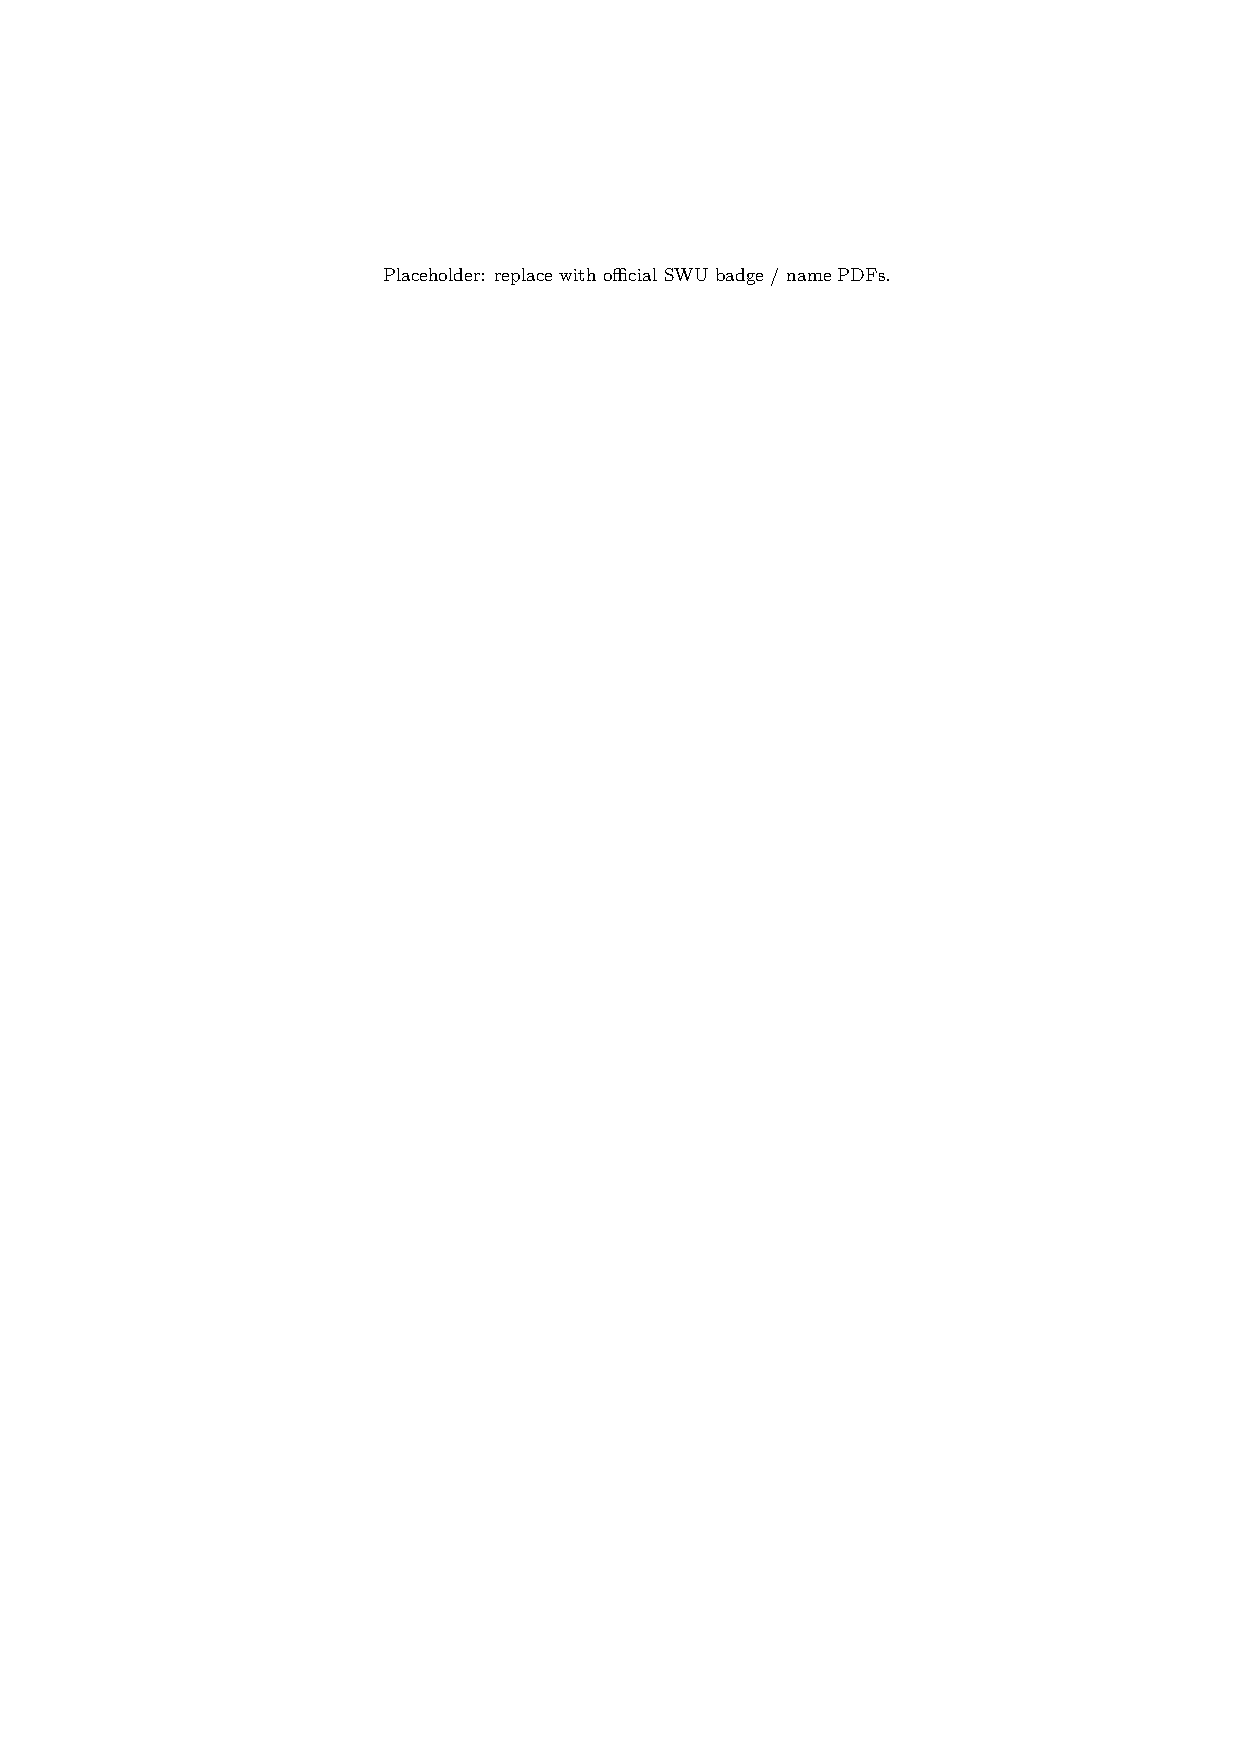
\includegraphics[width=0.88\textwidth,height=1.9cm,keepaspectratio]{figures/swu-name-stxingkai.pdf}\par
  \IfFileExists{figures/swu-name.pdf}{%
    \vspace{0.18\baselineskip}%
    \includegraphics[width=0.78\textwidth,height=0.7cm,keepaspectratio]{figures/swu-name.pdf}\par
  }{}%
}
% 封面校徽、校名图：宜为已裁去空白的 PDF；若整页 A4 仅含小图，仅用 |height=3.5cm| 缩放会使图在版心内几乎看不见。
% 左栏用 |width=\linewidth,height=3.5cm,keepaspectratio|，使图在栏宽内完整可见。
\newcommand{\swu@maketitle@doctor@zh}{%
  \begingroup
  \songti
  \noindent
  \begin{minipage}[t]{0.56\textwidth}
    \vspace{0pt}
    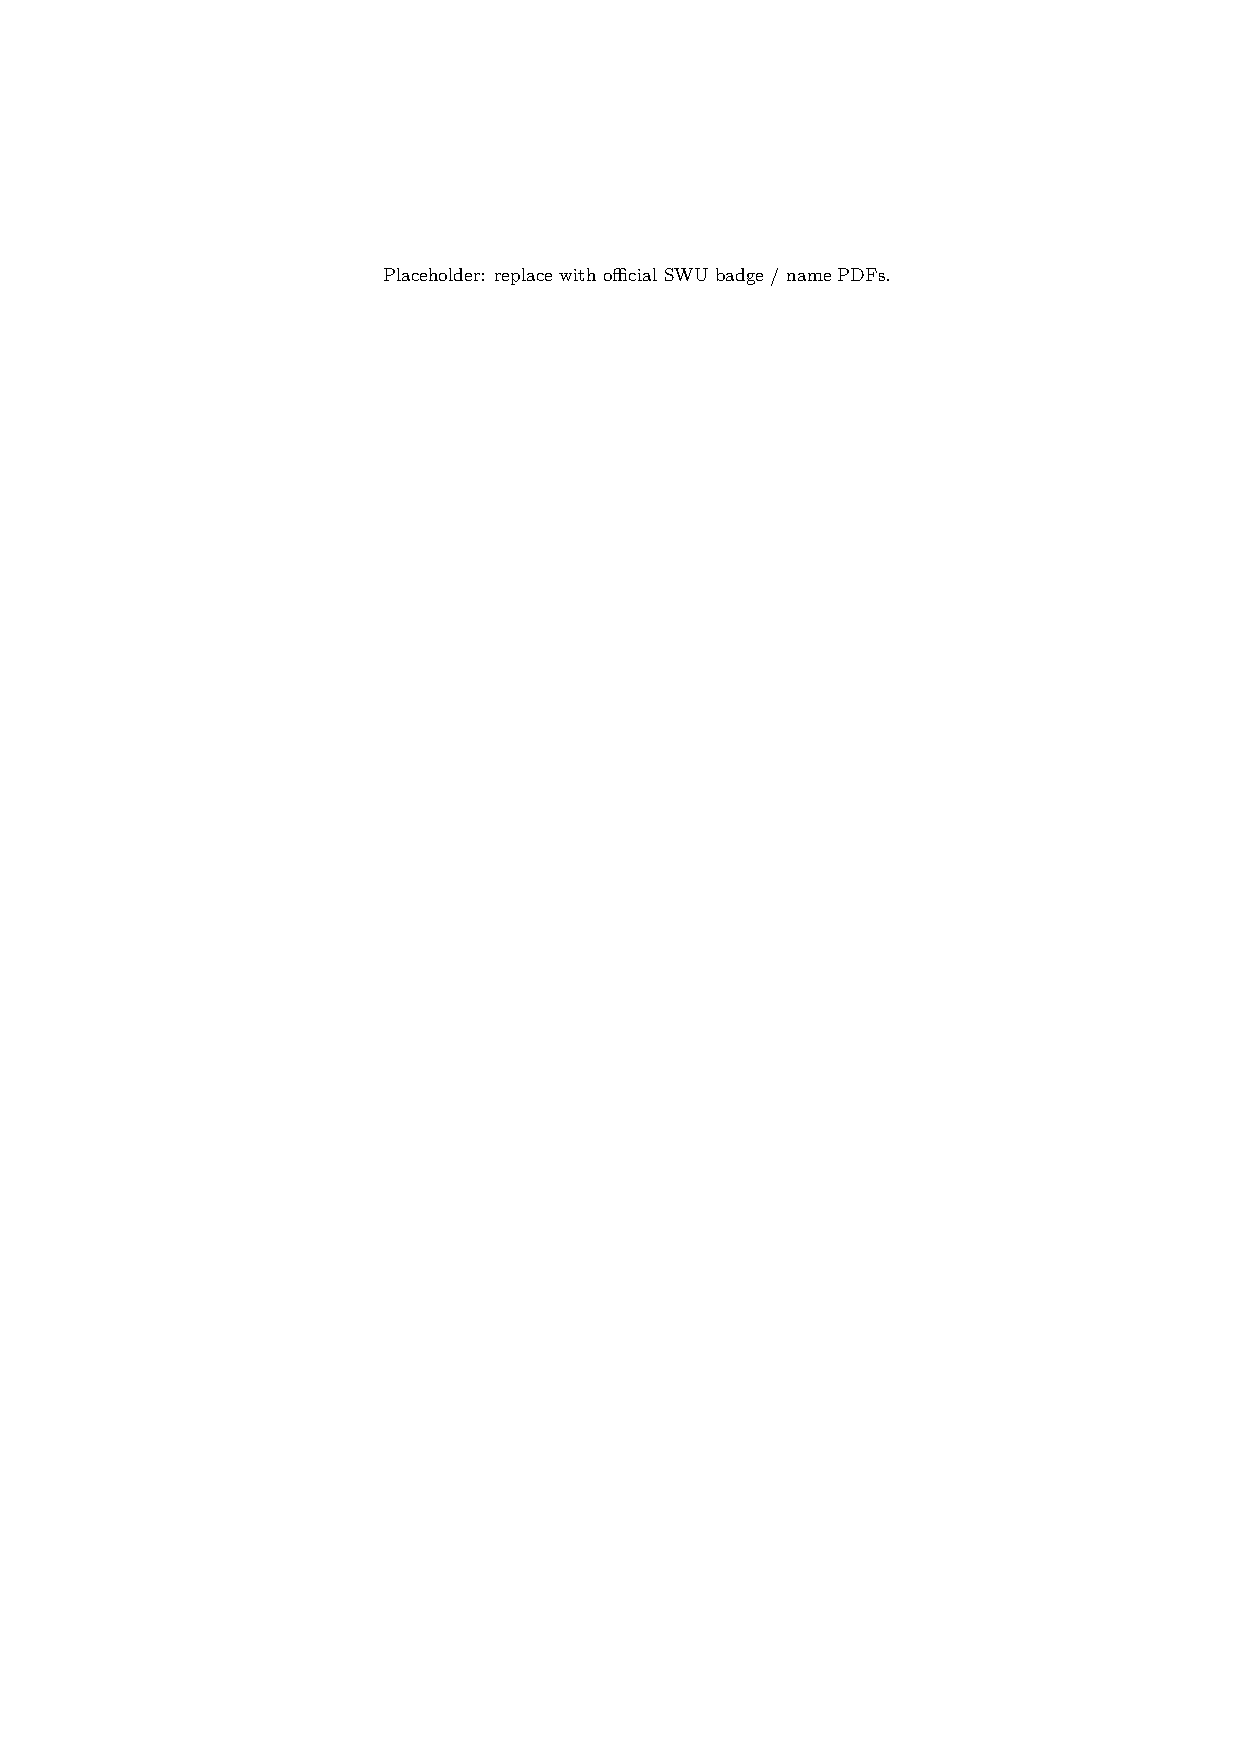
\includegraphics[width=\linewidth,height=3.5cm,keepaspectratio]{figures/swu-badge.pdf}%
  \end{minipage}
  \begin{minipage}[t]{0.44\textwidth}
    \vspace{0pt}
    \begin{flushright}
    \null\hfill
    {\zihao{4}%
    \begin{tabular}{@{}r@{\hspace{0.35em}}l@{}}%
      \makebox[4\ccwd][s]{\songti 单位代码}： & \songti\underline{\makebox[8\ccwd][c]{10635}} \\[0.42\baselineskip]
      \makebox[4\ccwd][s]{\songti 学　　号}： & \ttfamily\underline{\makebox[8\ccwd][c]{\swuStudentIdText}} \\
    \end{tabular}}%
    \end{flushright}
  \end{minipage}\par
  \begin{center}
    \swu@cover@schoolname@graphics
\vspace{-\baselineskip}
    {\youyuan\zihao{0}\bfseries \swuCJKStretchText{1.10}{博士学位论文}\par}
\vspace{1.2\baselineskip}
    {\zihao{2}\songti \swuTitleText\par}
    \swuSubtitleBlock
  \end{center}
  \vspace{1.8\baselineskip}
  {\centering\zihao{-3}\songti
    \swuCoverField{论文作者}{\swuAuthorText}
    \swuCoverField{指导教师}{\swuSupervisorText}
    \swuCoverField{学科专业}{\swuMajorText}
    \swuCoverField{研究方向}{\swuResearchFieldText}
    \swu@doctor@cover@date@single{提交日期}{%
      \swu@zh@date@inline{\swuSubmitYearText}{\swuSubmitMonthText}{\swuSubmitDayText}}%
    \swu@doctor@cover@date@single{答辩日期}{%
      \swu@zh@date@inline{\swuDefenseYearText}{\swuDefenseMonthText}{\swuDefenseDayText}}%
    \noindent\makebox[5\ccwd][s]{\bfseries 授予单位}：%
    \underline{\makebox[16\ccwd][c]{\kaishu 西南大学}}\par
    \vspace{0.6em}%
  }
  \vfill
  \begin{center}
    {\zihao{3}\youyuan\swuCJKStretchText{1.15}{中国重庆}\par}%
    \vspace{0.55\baselineskip}%
    {\zihao{3}\youyuan \swuDefenseYearText 年 \swuDefenseMonthText 月\par}%
  \end{center}%
  \vfill
  \endgroup
}
\newcommand{\swu@maketitle@doctor@en}{%
  \thispagestyle{empty}%
  \phantomsection
  \pdfbookmark[0]{英文题名页}{swu-title-en}%
  \begingroup
  \rmfamily
  \vspace*{0.4\baselineskip}%
  \begin{center}
    {\bfseries\zihao{2}\MakeUppercase{\swuTitleEnText}\par}%
    \vspace{0.85\baselineskip}%
    {\zihao{3}By\par}%
    \vspace{0.35\baselineskip}%
    {\bfseries\zihao{3}\MakeUppercase{\swuAuthorEnText}\par}%
    \vspace{0.82\baselineskip}%
    {\zihao{-4}A dissertation submitted to the\par}%
    \vspace{0.2\baselineskip}%
    {\zihao{-4}\swu@en@submitted@school\par}%
    \vspace{0.12\baselineskip}%
    {\zihao{-4}\swu@en@university\par}%
    \vspace{0.48\baselineskip}%
    {\zihao{-4}In partial fulfillment of the requirements\par}%
    \vspace{0.2\baselineskip}%
    {\zihao{-4}For the degree of\par}%
    \vspace{0.2\baselineskip}%
    {\zihao{-4}\swuDegreeEnText\par}%
    \expandafter\ifstrempty\expandafter{\swuGraduateProgramEnText}{%
      \expandafter\ifstrempty\expandafter{\swuCollegeEnText}{}{%
        \vspace{0.48\baselineskip}%
        {\zihao{-4}Graduate Program in \swuCollegeEnText\par}%
      }%
    }{%
      \vspace{0.48\baselineskip}%
      {\zihao{-4}\swuGraduateProgramEnText\par}%
    }%
    \vspace{0.38\baselineskip}%
    {\zihao{-4}Written under the direction of\par}%
    \vspace{0.2\baselineskip}%
    {\zihao{-4}\swu@graduate@supervisors@en\par}%
    \vspace{0.38\baselineskip}%
    {\zihao{-4}And approved by\par}%
    \swu@en@five@signature@lines
    \vfill
    \vspace{0.55\baselineskip}%
    {\zihao{-4}\swu@en@defense@location\par}%
    \vspace{0.25\baselineskip}%
    {\zihao{-4}\swu@en@defense@monthyear\par}%
    \vfill
  \end{center}%
  \endgroup
}
\newcommand{\makegraduateoriginalitystatement}{%
  \begingroup
  \songti\zihao{4}%
  \thispagestyle{empty}%
  \parindent=2\ccwd
  \phantomsection
  \pdfbookmark[0]{独创性声明与学位论文版权使用授权书}{swu-decl-grad-combined}%
  \begin{center}
    {\songti\bfseries\zihao{2}独创性声明}%
  \end{center}
  \vspace{0.4\baselineskip}
  \ignorespaces\swuGraduateTitleUnderlined
  \vspace{0.45\baselineskip}
  % 宋体四号（外层 |\songti\zihao{4}|），首行空两格（|\parindent=2\ccwd|）。
  本学位论文是作者在导师指导下独立完成的研究工作及取得的研究成果，恪守学术诚信，遵守学术准则。对本研究及学位论文撰写曾做出贡献的老师、朋友、同仁在文中作了明确说明并表示衷心感谢。\par
  \swuGraduateTwoPartySignatures
  \vspace{4\baselineskip}
  \begin{center}
    {\songti\bfseries\zihao{2}\swuCJKStretchText{1}{学位论文版权使用授权书}\par}
  \end{center}
  \vspace{0.4\baselineskip}
  \noindent\hspace*{2\ccwd}本学位论文作者完全了解西南大学有关保留、使用学位论文的规定，有权保留并向国家有关部门或机构送交论文的复印件和磁盘，允许论文被查阅和借阅。本人授权西南大学研究生院可以将学位论文的全部或部分内容编入有关数据库进行检索，可以采用影印、缩印或扫描等复制手段保存、汇编学位论文。\par
  \vspace{0.4\baselineskip}
  {\fangsong\zihao{4}\setlength{\parindent}{2\ccwd}%
  本论文公开时间：~ \swu@checkbox{}获学位当年； \swu@checkbox{}推迟1年； \swu@checkbox{}推迟2年。\par}%
  \swuGraduateTwoPartySignatures
  \endgroup
  \clearpage
}
%
\NewDocumentCommand{\maketitlepage}{}{
	\thispagestyle{empty}
	\phantomsection
	\pdfbookmark[0]{封面}{swu-cover}
	\ifswu@bachelor
	  \begingroup
	  \songti
	  \noindent
	  \begin{minipage}[t]{0.56\textwidth}
	    \vspace{0pt}
	    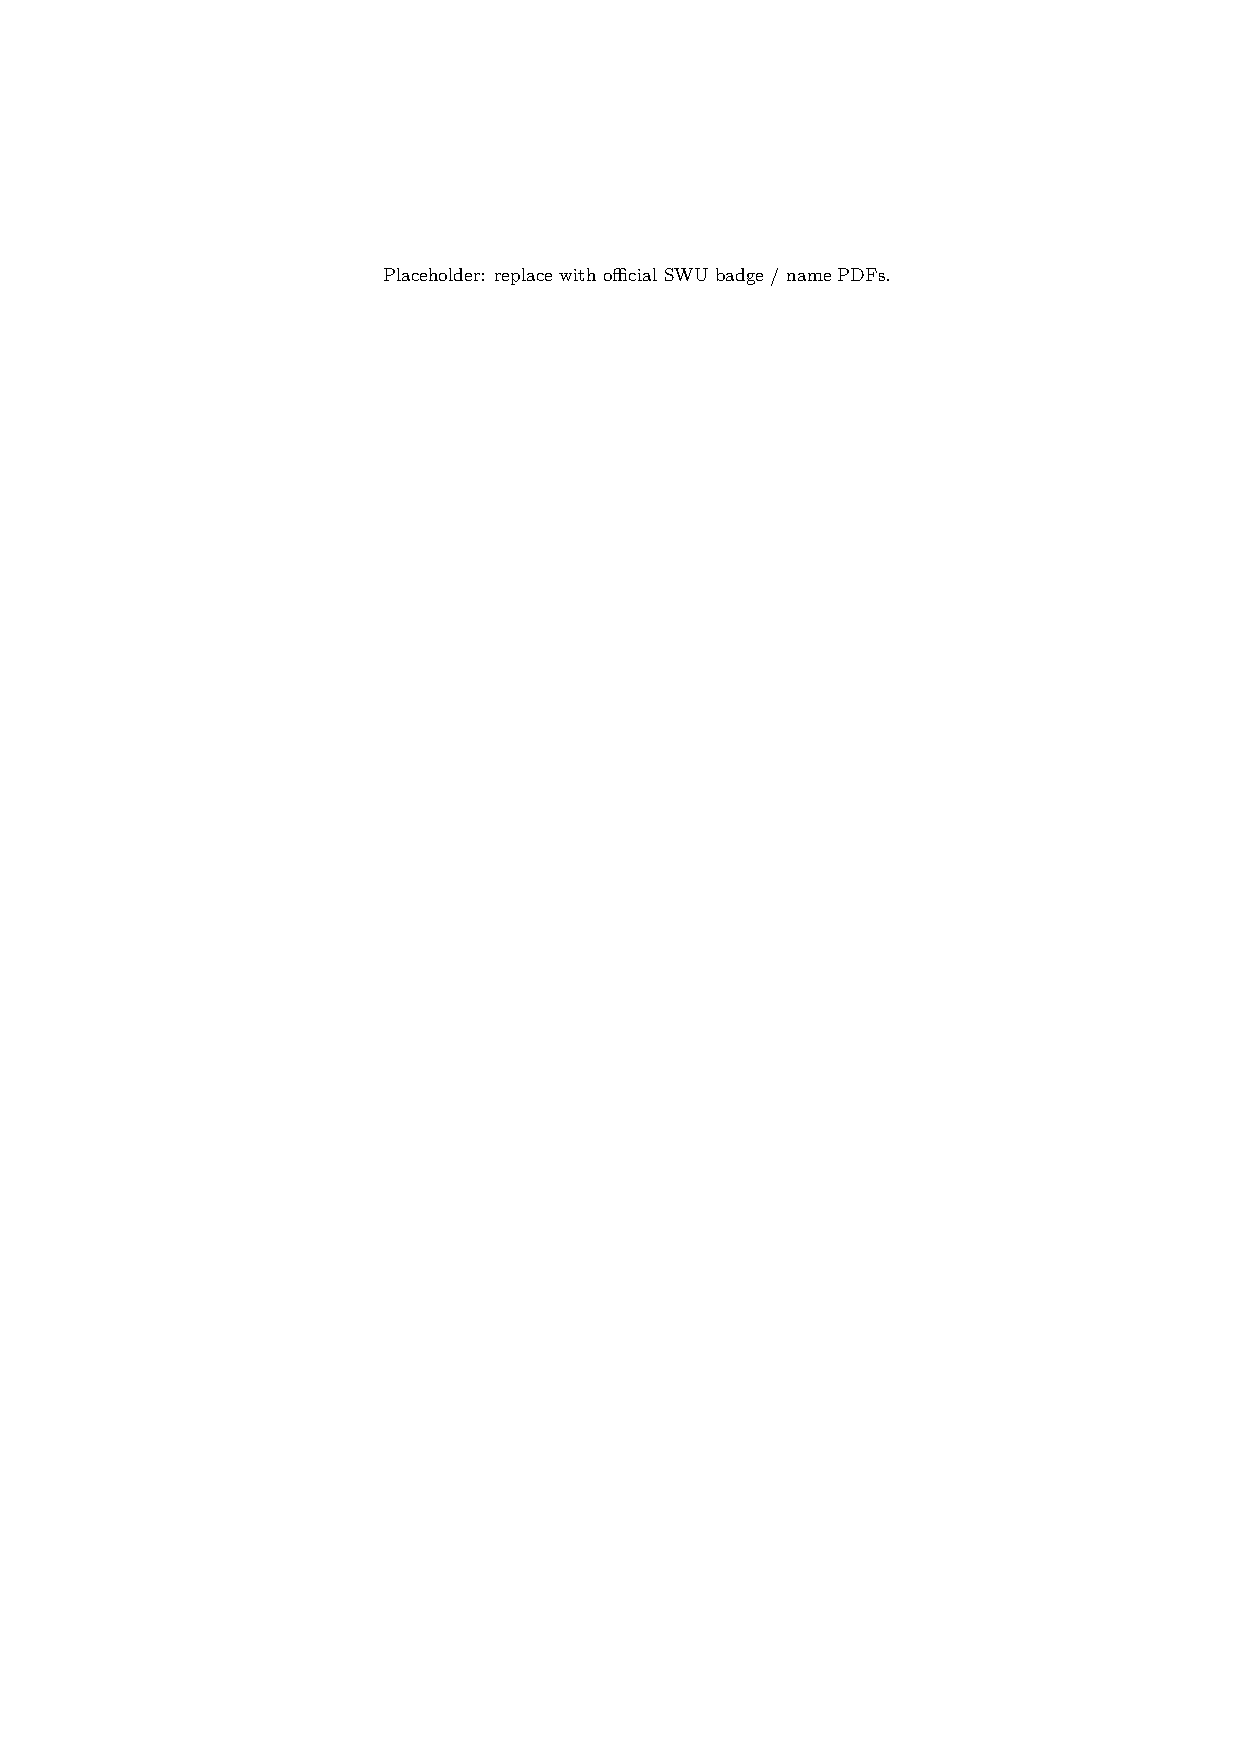
\includegraphics[width=\linewidth,height=3.5cm,keepaspectratio]{figures/swu-badge.pdf}%
	  \end{minipage}
	  \begin{minipage}[t]{0.44\textwidth}
	    \vspace{0pt}
	    \raggedleft{\zihao{4}\songti 单位代码：10635}
	  \end{minipage}\par
	  \begin{center}
	    \swu@cover@schoolname@graphics
		\vspace{-\baselineskip}
	    {\youyuan\zihao{0}\bfseries \swuCJKStretchText{1.10}{本科毕业论文（设计）}\par}
		\vspace{1.2\baselineskip}
	    {\zihao{2}\songti \swuTitleText\par}
	    \swuSubtitleBlock
	  \end{center}
	  \vspace{1.8\baselineskip}
	  {\centering\zihao{-3}\songti
	    \swuCoverField{学　　院}{\swuCollegeText}
	    \swuCoverField{专　　业}{\swuMajorText}
	    \swuCoverField{姓　　名}{\swuAuthorText}
	    \swuCoverField{学　　号}{\swuStudentIdText}
	    \swuCoverField{指导教师}{\swuSupervisorText}
	    \swuCoverField{答辩日期}{
	    \swuDefenseYearText 年
	    \swuDefenseMonthText 月
	    \swuDefenseDayText 日}\par
	  }
	  \vfill
	  \begin{center}
	    {\zihao{3}\youyuan \swuDefenseYearText 年 \swuDefenseMonthText 月\par}
	  \end{center}
	  \vfill
	  \endgroup
	  \clearpage
	  \makeoriginalitystatement
	\else
	  \ifswu@doctor
	    \swu@maketitle@doctor@zh
	    \clearpage
	    \swu@maketitle@doctor@en
	    \clearpage
	    \makegraduateoriginalitystatement
	  \else
	    \begin{center}
		    {\zihao{2}\bfseries 西南大学\swu@doctype\par}
		    \vspace{2cm}
		    {\zihao{2}\bfseries \swuTitleText\par}
		    \swuSubtitleBlock
		    \vspace{1.5cm}
		    {\zihao{4}作者：\swuAuthorText\par}
		    \vspace{0.5cm}
		    {\zihao{4}指导教师：\swuSupervisorText\par}
		    \vspace{0.5cm}
		    {\zihao{4}专业：\swuMajorText\par}
		    \vfill
		    {\zihao{4}\today\par}
	    \end{center}
	  \fi
	\fi
	\clearpage
}
% \texttt{book} 已定义 |\maketitle|（简易题名页）；本模板改为与 |\maketitlepage| 同义。
\renewcommand{\maketitle}{\maketitlepage}
%
\NewDocumentCommand{\makeabstract}{}{
	\clearpage
	\ifswu@gradthesis
	  \pagestyle{swugraduate}%
	  \thispagestyle{swugraduate}%
	\fi
	\phantomsection
	\addcontentsline{toc}{chapter}{摘要}
	\begin{center}
	  {\heiti\zihao{3}\swuTitleText\par}
	  \vspace{-0.5\baselineskip}
	  \swuSubtitleBlock
	  \vspace{0.3\baselineskip}
	  {\kaishu\zihao{-4}\swuAuthorText\par}
	  \vspace{0.3\baselineskip}
	  {\songti\zihao{5}西南大学\swuCollegeText，重庆 400715\par}
	\end{center}
	\vspace{\baselineskip}
	{\songti\zihao{5}\noindent\textbf{摘\hspace{1\ccwd}要：}%
	  \fangsong\swuAbstractCnText\par}
	{\songti\zihao{5}\noindent\textbf{关键词：}\swuKeywordsCnText\par}
	\vspace{2\baselineskip}
	\phantomsection
	\addcontentsline{toc}{chapter}{Abstract}
	\begin{center}
	  \vspace{\baselineskip}
	  {\rmfamily\bfseries\zihao{4}\swuTitleEnText\par}
	  \vspace{\baselineskip}
	  {\rmfamily\zihao{5}\swuAuthorEnText\par}
	  \vspace{0.5\baselineskip}
	  {\rmfamily\zihao{-5}\swuCollegeEnText, Southwest University,%
	    Chongqing 400715, PR China\par}
	\end{center}
	\vspace{\baselineskip}
	{\rmfamily\zihao{5}\noindent\textbf{Abstract: } \swuAbstractEnText\par}
	{\rmfamily\zihao{5}\noindent\textbf{Key words: } \swuKeywordsEnText\par}
}
%
\NewDocumentEnvironment{acknowledgements}{}{
	\clearpage
	\phantomsection
	\addcontentsline{toc}{chapter}{致\hspace{1\ccwd}谢}
	\begingroup
	\songti
	\setstretch{1}%
	\setlength{\parindent}{2\ccwd}%
	\setlength{\parskip}{0.5\baselineskip plus 0.2pt minus 0.2pt}%
	\begin{center}
	  {\songti\bfseries\zihao{-4}致\hspace{1\ccwd}谢\par}
	\end{center}
	\vspace{0.5\baselineskip}%
	\zihao{5}%
	\hspace{2\ccwd}\ignorespaces
}{\par\vspace{0.5\baselineskip}\endgroup}
%
\NewDocumentEnvironment{resume}{}{
	\chapter*{作者简介}
}{ }
%
\NewDocumentEnvironment{publications}{}{
	\clearpage
	\phantomsection
	\addcontentsline{toc}{chapter}{在读期间取得的科研成果}
	\begingroup
	\songti
	\setstretch{1}%
	\setlength{\parindent}{2\ccwd}%
	\setlength{\parskip}{0.5\baselineskip plus 0.2pt minus 0.2pt}%
	\begin{center}
	  {\songti\bfseries\zihao{-4}在读期间取得的科研成果\par}
	\end{center}
	\vspace{0.5\baselineskip}%
	\zihao{5}%
}{\par\vspace{0.5\baselineskip}\endgroup}
\newcommand{\swupublicationsubsection}[1]{%
	\par\vspace{\baselineskip}%
	\noindent
	{\songti\bfseries #1\par}%
	\vspace{0.35\baselineskip}%
}
\newenvironment{swupubenum}{%
	\begin{enumerate}[
		label={[\arabic*]},
		align=left,
		leftmargin=3.2em,
		labelsep=0.45em,
		itemsep=0.35\baselineskip,
		parsep=0pt,
		topsep=0.2\baselineskip
	]
}{
	\end{enumerate}%
}
\newcommand{\swu@defaultprintbibliography}{%
  \printbibliography[heading=bibintoc,%
    title={参考文献}]%
}
\newcommand{\swuprintbibliography}{\swu@defaultprintbibliography}
\makeatother
%</class>
%    \end{macrocode}
%
% \subsection{选项说明的推荐写法}
%
% 对于模板选项，建议采用“文档层说明 + 代码层声明”双轨写法：
% \begin{enumerate}
%   \item 在前文 ``用户接口概览'' 中，用自然语言解释用途；
%   \item 在实现部分，用 \verb|\DeclareBoolOption|、\verb|\DeclareVoidOption| 等给出正式定义；
%   \item 对互斥选项（如 postdoc/doctor/master/bachelor）补充优先级或默认规则说明。
% \end{enumerate}
%
% \subsection{命令说明的推荐写法}
%
% 对用户命令，推荐统一使用如下结构：
% \begin{verbatim}
% \DescribeMacro{\command}
% \verb|\command[<optional>]{<mandatory>}|
%
% 用法示例：
% \verb|\command{示例内容}|
%
% 功能说明
% 参数说明
% 注意事项
% \end{verbatim}
%
% \subsection{环境说明的推荐写法}
%
% 对环境，推荐统一使用如下结构：
% \begin{verbatim}
% \DescribeEnv{envname}
% \verb|\begin{envname}| ... \verb|\end{envname}|
%
% 使用示例：
% \verb|\begin{envname} 示例内容 \end{envname}|
%
% 功能说明
% 环境体内容要求
% 与章节命令的关系
% \end{verbatim}
%
% \section{维护建议}
%
% 建议将整个模板拆为以下层次：
% \begin{itemize}
%   \item 文档类主文件：\texttt{swuthesis.cls}；
%   \item 学位层选项模块：博士后/博士/硕士/本科；
%   \item 页面与封面模块；
%   \item 摘要、目录、参考文献、附录模块；
%   \item 用户接口文档模块。
% \end{itemize}
%
% \subsection{各学位实现状态（便于后续扩展）}
%
% 截至当前版本，类选项 \texttt{postdoc}、\texttt{doctor}、\texttt{master}、\texttt{bachelor}
% 已声明，且 |\swu@doctype| 会随选项切换题名用语；但\textbf{版式实现程度并不相同}：
% \begin{description}
%   \item[bachelor] 封面（含校徽、题名行、学院/专业等字段）、独创声明与授权声明、
%         中英文摘要页等，已按本科常见版式实现；示例主文档 \texttt{swuthesis-main.tex} 以此为准。
%   \item[doctor] 已提供中文封面（与本科共用校徽、校名图片及单位代码版式）、英文题名页、
%         独创性声明与学位论文版权使用授权书（研究生院版双签栏与公开时间选项；题目取自 |\swusetup| 的 |title|）；
%         |\swusetup| 增加 |research-field|、|degree-en|、|supervisor-en| 等键。
%         若研究生院修订表格文本，请直接修改 |swuthesis.dtx| 中 |\makegraduateoriginalitystatement| 对应段落。
%   \item[master / postdoc] |\maketitlepage| 中非本科分支仍为\textbf{占位式}题名页
%         （居中标题、作者、导师、专业、|\today|）；|\makeabstract| 目前与各学位共用同一摘要版式，
%         若规范要求分学位调整，宜拆分为内部命令再对外保留 |\makeabstract|。
%   \item[选项组合] 互斥选项（四选一）尚未在代码层强制校验；若同时传入多个布尔选项，可能得到
%         意料之外的 |\swu@doctype| 与分支结果。后续可约定「仅允许一个学位选项」或「默认本科、
%         显式指定研究生」等规则，并在 |\ProcessKeyvalOptions| 之后用
%         |\PackageWarning|/|\PackageError| 提示。
% \end{description}
% 环境 |publications| 标题为「在读期间取得的科研成果」，博士后或外校规范若需改标题，
% 可在后续版本增加键值选项；小标题与分条编号见 |\swupublicationsubsection| 与 |swupubenum|。
%
% 若模板后续复杂度提高，可在 \texttt{.dtx} 中使用多个 guard，例如
% \texttt{<*class>}、\texttt{<*cfg>}、\texttt{<*example>}，从而抽取多个文件。

% \subsection{示例文档抽取}
%
% 运行 \texttt{latex swuthesis.ins} 除抽取类文件外，还会生成本科示例 \path{swuthesis-main.tex} 与
% 博士示例 \path{swuthesis-doctor-main.tex}（后者由 \texttt{doctor} 抽取块生成；维护时请编辑 \path{swuthesis.dtx} 中对应段落）。
%
% 示例中的 \texttt{swuthesis-main.bib} 由 \verb|filecontents*| 生成；条目著录与公开书目一致，
% 并覆盖国标、西文专著、\texttt{CTeX} 手册、中文专著与期刊（可在 CNKI 等检索）、
% MathSciNet 著录的数学期刊论文、arXiv 预印本与 NeurIPS 会议论文等类型；键名与
% \texttt{references.bib} 中部分条目对齐，便于对照维护。
%
%    \begin{macrocode}
%<*example>
\begin{filecontents*}[overwrite]{swuthesis-main.bib}
@standard{gbt7714,
  title        = {信息与文献 参考文献著录规则},
  organization = {国家市场监督管理总局、国家标准化管理委员会},
  number       = {GB/T 7714---2025},
  year         = {2025},
  address      = {北京},
  publisher    = {中国标准出版社}
}

@book{knuth1984texbook,
  author    = {Donald E. Knuth},
  title     = {The {\TeX}book},
  volume    = {A},
  series    = {Computers and Typesetting},
  publisher = {Addison-Wesley},
  year      = {1984},
  address   = {Reading, MA}
}

@book{lamport1994latex,
  author    = {Leslie Lamport},
  title     = {{\LaTeX}: A Document Preparation System},
  edition   = {2},
  publisher = {Addison-Wesley},
  year      = {1994},
  address   = {Reading, MA}
}

@book{mittelbach2004companion,
  author    = {Frank Mittelbach and Michel Goossens and Johannes Braams and David Carlisle},
  title     = {The {\LaTeX} Companion},
  edition   = {2},
  publisher = {Addison-Wesley},
  year      = {2004},
  address   = {Boston}
}

@manual{ctex2022,
  title        = {{CTeX} 宏集手册},
  author       = {{CTeX-org}},
  organization = {CTeX-org},
  year         = {2022},
  note         = {CTAN: https://ctan.org/pkg/ctex. 引用日期: 2026-04-18.},
  langid       = {chinese}
}

@book{zhouzhihua2016ml,
  author    = {周志华},
  title     = {机器学习},
  publisher = {清华大学出版社},
  year      = {2016},
  address   = {北京},
  isbn      = {978-7-302-42328-7},
  langid    = {chinese}
}

@article{liguojie2012bigdata,
  author       = {李国杰 and 程学旗},
  title        = {大数据研究: 未来科技及经济社会发展的重大战略领域——大数据的研究现状与科学思考},
  journaltitle = {中国科学院院刊},
  year         = {2012},
  volume       = {27},
  number       = {6},
  pages        = {647--657},
  issn         = {1000-3045},
  langid       = {chinese}
}

@article{WalpuskiZhang2021DMJ,
  author       = {Walpuski, Thomas and Zhang, Boyu},
  title        = {On the Compactness Problem for a Family of Generalized {Seiberg--Witten} Equations in Dimension 3},
  journaltitle = {Duke Mathematical Journal},
  shortjournal = {Duke Math. J.},
  volume       = {170},
  number       = {17},
  pages        = {3891--3934},
  year         = {2021},
  doi          = {10.1215/00127094-2021-0005},
  note         = {MathSciNet MR4340726},
  langid       = {english}
}

@misc{taubes2020compactness,
  author     = {Taubes, Clifford Henry},
  title      = {{Compactness theorems for $\mathrm{SL}(2;\mathbb{C})$ generalizations of the 4-dimensional anti-self dual equations}},
  year       = {2020},
  eprinttype = {arxiv},
  eprint     = {1307.6447},
  langid     = {english}
}

@inproceedings{vaswani2017attention,
  author    = {Vaswani, Ashish and Shazeer, Noam and Parmar, Niki and Uszkoreit, Jakob and Jones, Llion and Gomez, Aidan N. and Kaiser, {\L}ukasz and Polosukhin, Illia},
  title     = {Attention Is All You Need},
  booktitle = {Advances in Neural Information Processing Systems 30: Proceedings of the 31st Conference on Neural Information Processing Systems},
  year      = {2017},
  pages     = {5998--6008},
  publisher = {Curran Associates, Inc.},
  address   = {Long Beach, CA, USA},
  langid    = {english}
}

@online{swu2021thesisManageNotice,
  author    = {{西南大学}},
  title     = {关于印发《西南大学全日制本科学生毕业论文（设计）工作管理办法》的通知},
  date      = {2021-01-07},
  url       = {https://ceie.swu.edu.cn/info/1125/3918.htm},
  urldate   = {2026-04-18},
  note      = {西校〔2021〕4号},
  langid    = {chinese}
}

@online{swuUndergradThesisSpecWeb,
  author    = {{西南大学}},
  title     = {西南大学本科毕业论文（设计）规范},
  url       = {https://ceie.swu.edu.cn/__local/B/91/38/9FF7435A5836B7EB071487AD731_A201FE06_1F75D.docx?e=.docx},
  urldate   = {2026-04-18},
  langid    = {chinese}
}

@online{swu2022gradThesisSpecDoc,
  author    = {{西南大学}},
  title     = {西南大学博士硕士学位论文规范},
  date      = {2022-06-28},
  url       = {https://dwyx.swu.edu.cn/info/1083/2038.htm},
  urldate   = {2026-04-18},
  note      = {西南大学博士硕士学位论文规范.doc},
  langid    = {chinese}
}

@misc{bao2024swuthesisLegacy,
  author       = {包小敏},
  title        = {西南大学本科毕业论文 {\LaTeX} 模板（本科毕业论文模板\_新）},
  year         = {2024},
  month        = aug,
  howpublished = {西南大学数学与统计学院本科毕业论文写作模板；含 myTemplate.tex、SWUthesis.sty 等},
  note         = {持续维护至 2024 年；联系信箱 xbao@swu.edu.cn},
  langid       = {chinese}
}
\end{filecontents*}

\documentclass[bachelor,fontset=macnew, punct=banjiao]{swuthesis}

\usepackage{subcaption}
\usepackage{longtable}
\usepackage{siunitx}
\usepackage{tikz}
\usetikzlibrary{arrows.meta,positioning}
\sisetup{detect-all}

\swusetup{
  title         = {西南大学本科毕业论文模板示例文档},
  subtitle      = {基于 \texttt{swuthesis.dtx} 自动生成的主文档},
  title-en      = {An Example Main Document Generated from \texttt{swuthesis.dtx}},
  college       = {数学与统计学院},
  college-en    = {School of Mathematics and Statistics},
  major         = {数学与应用数学},
  author        = {张三},
  author-en     = {San Zhang},
  student-id    = {222026314210000},
  supervisor    = {李四\ 教授},
  defense-year  = {2026},
  defense-month = {6},
  defense-day   = {18}
}

\addbibresource{swuthesis-main.bib}

\begin{document}

\frontmatter
\maketitle
\tableofcontents
\begin{cnabstract}
本文给出一个面向西南大学本科毕业论文（设计）的 \LaTeX{} 模板示例文档，
重点演示封面与摘要生成、章节结构组织、插图与子图排版、三线表与长表格排版、数学公式编号与引用、
定理环境定义以及参考文献著录等常见功能。示例内容同时吸收学校现行本科毕业论文（设计）规范中的
基本要求、编写格式、排版要求和材料装袋顺序，用于说明如何将正式规范转化为可复用的模板结构。
该示例既可作为模板测试文件，也可作为后续扩展博士、硕士与本科统一文档体系的基础。
附录收录《西南大学本科毕业论文（设计）规范》全文，便于对照。
\end{cnabstract}
\begin{cnkeywords}
西南大学；毕业论文模板；\LaTeX；本科论文；排版示例
\end{cnkeywords}
\begin{enabstract}
This document presents an undergraduate thesis example for Southwest University
based on \LaTeX. It demonstrates the generation of the cover page and bilingual abstract,
chapter organization, figures and aligned subfigures, three-line tables and long tables,
equation numbering and cross-referencing, theorem-like environments, and bibliography formatting.
The example also incorporates the current undergraduate thesis specification of the university,
so that formal writing requirements can be translated into a reusable template structure.
It is intended both as a regression test for the class file and as a starting point for a unified
document system covering undergraduate, master's, and doctoral theses.
\end{enabstract}
\begin{enkeywords}
Southwest University; thesis template; \LaTeX; undergraduate thesis; typesetting example
\end{enkeywords}
\makeabstract

\mainmatter
\chapter{模板制作说明}\label{ch:guide}

本章说明本示例文档的用途，以及模板与学校正式规范之间的关系。《西南大学本科毕业论文（设计）规范》为统一本科毕业论文（设计）的撰写和编辑格式，保证本科毕业论文（设计）的质量，便利信息系统的收集加工、检索利用和交流传播，在《西南大学全日制本科学生毕业论文（设计）工作管理办法》（西校〔2021〕4号）基础上制定\cite{swu2021thesisManageNotice,swuUndergradThesisSpecWeb}。\textbf{该规范的完整条文已收录于附录~\ref{app:swu-undergrad-spec}}，写作与提交时请以学校最新发布的文件为准；若规范修订，请相应更新附录文本或改附说明。博士、硕士学位论文的撰写与排版另有《西南大学博士硕士学位论文规范》\cite{swu2022gradThesisSpecDoc}（页面提供 \texttt{.doc} 文档下载，以学校及学院最新发布为准）。

\section{编译与工具链}\label{sec:compile}
\subsection{引擎与参考文献后端}
正文为中文并依赖字体与 \texttt{ctex}，\textbf{须使用 \hologo{XeLaTeX}} 编译。参考文献使用 \texttt{biblatex}，\textbf{须运行 \hologo{biber}}（随 TeX~Live、MiKTeX 等发行版安装，版本号随发行版更新；与 \texttt{biblatex} 配套的是名为 \hologo{biber} 的程序，在编辑器中配置「参考文献处理器」时选 \hologo{biber} 即可）。\textbf{不要使用}以 \hologo{pdfLaTeX} 为默认的一键流程（例如 WinEdt 中常见的 PDF\TeX{}ify），否则无法正确排版中文与参考文献。

\subsection{Windows（含 WinEdt）}
\begin{itemize}
  \item \textbf{Biber 与 WinEdt}：WinEdt 不单独「支持某个 biber 版本号」，而是调用发行版已安装的 \hologo{biber}（Windows 下可执行文件名为 \texttt{biber.exe}）。在 \texttt{TeX} $\rightarrow$ \texttt{Execution Modes}（或同类菜单）中，将主流程设为 \textbf{\hologo{XeLaTeX}}，并在需要时增加一步 \hologo{biber}，再多次 \hologo{XeLaTeX}，顺序与下文 Makefile 一致即可。
  \item \textbf{避免 PDF\TeX{}ify}：该快捷方式通常绑定 \hologo{pdfLaTeX}，与本模板不兼容。请改用「\hologo{XeLaTeX} + \hologo{biber} + \hologo{XeLaTeX}」或下文 \texttt{latexmk}。
  \item 若已安装 TeX~Live 并将 \texttt{bin} 加入系统 \texttt{PATH}，也可在「命令提示符」或 PowerShell 中进入工程目录，手动执行与 \cref{sec:compile-make} 相同的命令。
\end{itemize}

\subsection{macOS / Linux 与 \texttt{Makefile}}\label{sec:compile-make}
工程根目录的 \path{Makefile} 会依次执行：\hologo{XeLaTeX} $\rightarrow$ \hologo{biber} $\rightarrow$ \hologo{XeLaTeX} $\rightarrow$ \hologo{XeLaTeX}（与参考文献、交叉引用完全刷新所需次数一致）。在终端进入工程目录后执行 \texttt{make} 或 \texttt{make main} 即可。\textbf{\texttt{make} 为系统自带或随「构建工具」安装}：macOS 若提示无此命令，可安装 Xcode Command Line Tools（终端执行 \texttt{xcode-select --install}）；Linux 可通过包管理器安装 \texttt{make} 或 \texttt{build-essential}。无需单独「安装 Makefile」这一软件——只需 \texttt{make} 程序与已安装的 \TeX{} 发行版。

\subsection{持续编译（\texttt{latexmk}）}
TeX~Live 等发行版自带 \texttt{latexmk}，可根据辅助文件自动决定运行次数及是否调用 \hologo{biber}。写作时可在工程目录使用「监视文件并反复编译」：
\begin{verbatim}
latexmk -pvc -xelatex swuthesis-main.tex
\end{verbatim}
选项 \texttt{-pvc} 表示持续预览（源文件保存后自动重新编译）。若工程根目录提供 \path{.latexmkrc}（本仓库已含），其中已将引擎设为 \hologo{XeLaTeX}，亦可简写为 \texttt{latexmk -pvc swuthesis-main.tex}。首次编译前请已生成 \path{swuthesis.cls}（例如运行 \texttt{latex swuthesis.ins} 或 \texttt{make cls}）。

\section{与既有本科毕业论文模板的关系及本模板的必要性}
西南大学本科论文写作中长期流传着一类以 \textsf{ctexbook} 为主文档类、以 \path{SWUthesis.sty} 为版式与宏包集合、用 \texttt{\textbackslash include} 分文件组织封面、声明、摘要与正文的模板（例如目录中常出现 \path{myTemplate.tex}、\path{preample/coverpage.tex} 等结构，坊间多称「本科毕业论文模板\_新」一类资源；可参考文献\cite{bao2024swuthesisLegacy}）。

其在\textbf{工作流程}（封面—声明—目录—中英文摘要—分章正文—参考文献—附录）与\textbf{版式目标}（本科论文常见章节划分）上，为本项目提供了\textbf{部分经验参考}。

本仓库中的 \texttt{swuthesis} 并非在上述 \texttt{.sty} 源码上逐行修补，而是\textbf{全新设计}的文档类：以 \path{swuthesis.dtx} 生成 \path{swuthesis.cls}，用 \LaTeX3 键值接口集中论文元信息，参考文献采用 \texttt{biblatex} 与 GB/T~7714 系列样式，定理与交叉引用等与当前 \TeX{} Live 生态对齐。这样做的必要性在于：
\begin{enumerate}[label=\arabic*., leftmargin=2em]
  \item \textbf{可维护性与可重复构建}：单一类文件 + 主文档，版本信息清晰，便于随学校规范修订而更新；减少「个人魔改 sty、他人环境无法编译」的风险。
  \item \textbf{与现代工具链一致}：避免依赖已弱化或停更的宏包组合（如部分早期插图、表格与中文下划线方案），降低在新系统上的故障率。
  \item \textbf{扩展空间}：同一套类文件可继续向硕士、博士或学院细则分支演进，而不必在多个分散的 \texttt{\textbackslash include} 工程中重复同步版式。
\end{enumerate}
因此：旧模板可作为\textbf{使用习惯与目录结构}的参照；本模板则面向\textbf{长期维护、规范对齐与协作}，二者是\textbf{继承目标、重新实现}的关系，而非简单的「换皮」或补丁升级。

\section{示例文档的定位}
\texttt{swuthesis} 示例用于检验类文件与主文档能否正确生成封面、中英文摘要、目录、章节、图表、公式、定理环境与参考文献列表等。\LaTeX{} 负责版式与自动化，\textbf{不能替代}对选题、方法与学术规范的理解。

\section{与学校规范的关系}
学校对字数、结构、参考文献、装袋材料等有统一要求。正文各章演示排版命令的用法；\textbf{条文级全文}见附录~\ref{app:swu-undergrad-spec}。学院若有补充规定，以学院通知为准。

\section{阅读与修改建议}
撰写真实论文时，建议先通读附录中的规范，再按学院模板整理材料；使用本模板时，可在导言区按需载入宏包，但不宜改动学校规定的封面与声明页要素。

\section{程序代码与 \texttt{listings}}\label{sec:code-inclusion}
\texttt{swuthesis} 已载入 \texttt{listings} 并定义代码样式。正文中可使用 \texttt{\textbackslash lstinline}、\texttt{lstlisting} 环境或 \texttt{\textbackslash lstinputlisting} 从子目录引入源码。
Matlab、Wolfram 语言（\texttt{listings} 中标识为 \texttt{Mathematica}）、Python、R、C++ 等示例见附录~\ref{app:code-matlab}--\ref{app:code-cpp}。

\paragraph{附录示例来源说明}
文末附录设有标题为\textbf{附录示例来源说明}的一节（见\hyperref[app:source-note]{该处}），专门说明上述程序附录与先行模板、包小敏老师维护工作及文献\cite{bao2024swuthesisLegacy} 之间的关系。正式撰写毕业论文时，若使用或改写此类示例代码，建议保留相应说明或在致谢中予以说明。

\chapter{插图}\label{ch:figures}

\section{使用 \texttt{graphicx} 插入外部图片}
日常插图可将图形文件（如 \path{.pdf}、\path{.png}、\path{.jpg}）置于工程目录下，用 \texttt{\textbackslash includegraphics} 插入。
以下使用 \TeX{} Live 等发行版自带的示例图 \path{example-image-a}、\path{example-image-b}、\path{example-image-c}（由 \textsf{mwe} 宏包提供，无需复制到工程目录），便于在无自备图片时也能编译通过；实际写作时替换为自有文件名即可。

\subsection{单幅图}
\begin{figure}[htbp]
  \centering
  \includegraphics[width=0.55\textwidth]{example-image-a}
  \caption{单幅插图示例（\texttt{example-image-a}）}
  \label{fig:graphicx-single}
\end{figure}

\subsection{左右子图}
\begin{figure}[htbp]
  \centering
  \begin{subfigure}[b]{0.47\textwidth}
    \centering
    \includegraphics[width=\linewidth]{example-image-b}
    \caption{左侧子图}
    \label{fig:graphicx-sub-left}
  \end{subfigure}
  \hfill
  \begin{subfigure}[b]{0.47\textwidth}
    \centering
    \includegraphics[width=\linewidth]{example-image-c}
    \caption{右侧子图}
    \label{fig:graphicx-sub-right}
  \end{subfigure}
  \caption{左右子图排版示例（\texttt{example-image-b} 与 \texttt{example-image-c}）}
  \label{fig:graphicx-subfigures}
\end{figure}

由 \cref{fig:graphicx-single,fig:graphicx-subfigures} 可见，图题置于图下方；子图环境使用相同宽度并采用 \texttt{[b]} 选项可实现底部对齐，各子图有独立子题与引用标签。

\section{TikZ 绘图示例}
需要流程图、示意图等矢量图时，可使用 \textsf{tikz} 在源码中直接绘制（编译较慢，适合简单图形）。

\subsection{流程示意图}
\begin{figure}[htbp]
  \centering
  \begin{tikzpicture}[node distance=18mm,>=Latex]
    \node[draw,rounded corners,minimum width=25mm,minimum height=10mm] (spec) {学校规范};
    \node[draw,rounded corners,right=of spec,minimum width=25mm,minimum height=10mm] (class) {类文件};
    \node[draw,rounded corners,right=of class,minimum width=25mm,minimum height=10mm] (main) {主文档};
    \draw[->,thick] (spec) -- (class);
    \draw[->,thick] (class) -- (main);
  \end{tikzpicture}
  \caption{模板生成流程示意图（TikZ）}
  \label{fig:tikz-workflow}
\end{figure}

\subsection{并列示意子图}
\begin{figure}[htbp]
  \centering
  \begin{subfigure}[b]{0.47\textwidth}
    \centering
    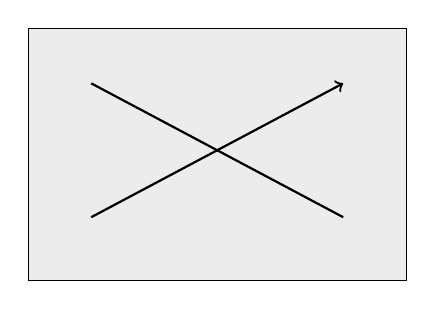
\begin{tikzpicture}
      \draw[fill=gray!15] (0,0) rectangle (4.8,3.2);
      \draw[thick,->] (0.8,0.8) -- (4,2.5);
      \draw[thick] (0.8,2.5) -- (4,0.8);
    \end{tikzpicture}
    \caption{简单示意子图}
    \label{fig:tikz-sub-left}
  \end{subfigure}
  \hfill
  \begin{subfigure}[b]{0.47\textwidth}
    \centering
    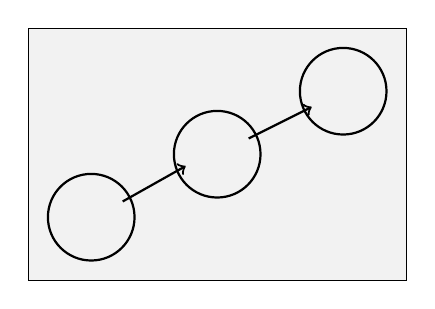
\begin{tikzpicture}
      \draw[fill=gray!10] (0,0) rectangle (4.8,3.2);
      \draw[thick] (0.8,0.8) circle [radius=0.55];
      \draw[thick] (2.4,1.6) circle [radius=0.55];
      \draw[thick] (4.0,2.4) circle [radius=0.55];
      \draw[thick,->] (1.2,1.0) -- (2.0,1.45);
      \draw[thick,->] (2.8,1.8) -- (3.6,2.2);
    \end{tikzpicture}
    \caption{并列对齐子图}
    \label{fig:tikz-sub-right}
  \end{subfigure}
  \caption{左右两个子图排版示例（TikZ）}
  \label{fig:tikz-subfigures}
\end{figure}

\cref{fig:tikz-workflow,fig:tikz-subfigures} 与上文 \texttt{graphicx} 示例的版式要求一致：图题在图下、子图可对齐引用。

\chapter{表格}\label{ch:tables}

\section{三线表示例}
\begin{table}[htbp]
  \centering
  \caption{模板常用环境与用途}
  \label{tab:booktabs}
  \begin{tabular}{lll}
    \toprule
    环境或命令 & 主要用途 & 备注 \\
    \midrule
    \texttt{\textbackslash chapter} & 一级结构组织 & 自动编号 \\
    \texttt{figure} & 插图排版 & 图题置底 \\
    \texttt{table} & 表格排版 & 表题置顶 \\
    \texttt{equation} & 单行公式 & 可交叉引用 \\
    \texttt{theorem} & 定理类内容 & 按章编号 \\
    \bottomrule
  \end{tabular}
\end{table}

\section{长表格示例}
\begin{center}
\begin{longtable}{clp{0.55\textwidth}}
  \caption{本科毕业论文（设计）组成部分说明}\\
  \toprule
  序号 & 组成部分 & 说明 \\
  \midrule
  \endfirsthead
  \caption[]{本科毕业论文（设计）组成部分说明（续）}\\
  \toprule
  序号 & 组成部分 & 说明 \\
  \midrule
  \endhead
  \bottomrule
  \endfoot
  1 & 封面 & 使用学校统一格式，体现题目、学院、专业、姓名、学号和指导教师等信息。 \\
  2 & 独创声明与授权书 & 每本论文均应附有声明页，并保留本人手写签名。 \\
  3 & 目录 & 一般列到二级标题，目录页码单独编排。 \\
  4 & 中英文摘要 & 中文在前，英文在后，需含标题、作者、单位、摘要与关键词。 \\
  5 & 导论或引言 & 交代问题背景、研究意义、研究目的和研究现状。 \\
  6 & 正文 & 论文核心部分，可根据研究内容划分多个章节。 \\
  7 & 结论 & 应准确、完整、精练，不应只是正文小结的重复。 \\
  8 & 参考文献 & 应选取查阅过且具有参考价值的权威文献，数量与外文比例须满足学校要求。 \\
  9 & 致谢 & 仅限于对论文完成有较大帮助的单位和个人。 \\
  10 & 附录 & 用于放置补充性的图表、程序、问卷或原始数据，非必须部分。 \\
\end{longtable}
\end{center}

\chapter{数学公式}\label{ch:math}

\section{编号与对齐}
模板已按章对公式编号，且可直接使用 \texttt{\textbackslash label} 与 \texttt{\textbackslash cref} 进行交叉引用。
例如，线性回归的最小二乘目标函数可写为
\begin{equation}
  J(\boldsymbol{\beta})=\lVert \mathbf{y}-\mathbf{X}\boldsymbol{\beta} \rVert_2^2.
  \label{eq:objective}
\end{equation}
对参数求导并令其为零，可得正规方程
\begin{align}
  \frac{\partial J}{\partial \boldsymbol{\beta}}
  &= -2\mathbf{X}^{\mathsf T}\left(\mathbf{y}-\mathbf{X}\boldsymbol{\beta}\right)=0, \label{eq:gradient}\\
  \mathbf{X}^{\mathsf T}\mathbf{X}\boldsymbol{\beta}
  &= \mathbf{X}^{\mathsf T}\mathbf{y}. \label{eq:normal}
\end{align}
由 \cref{eq:objective,eq:gradient,eq:normal} 可见，单公式和对齐公式都能正确编号和引用。

考虑方程组
\begin{equation}\label{eq:uniform}
\begin{aligned}
  a\cos\theta+b\sin\theta&=10,\\
  b\cos\theta+a\sin\theta&=10
\end{aligned}
  \implies a^2+b^2=100.
\end{equation}
\eqref{eq:uniform}实现了统一编号。
\section{常见数学符号排版}
下列公式展示了常见的集合、极限、求和、积分和矩阵写法：
\begin{equation}
  A=\left\{x\in\mathbb{R}: x^2\le 1\right\}, \qquad
  \lim_{n\to\infty}\sum_{k=1}^{n}\frac{1}{k^2}=\frac{\pi^2}{6}.
\end{equation}
\begin{equation}
  \int_{0}^{1} x^\alpha (1-x)^\beta\,\mathrm{d}x
  = \frac{\Gamma(\alpha+1)\Gamma(\beta+1)}{\Gamma(\alpha+\beta+2)}.
\end{equation}
\begin{equation}
  \mathbf{A}=
  \begin{bmatrix}
    1 & 0 & 2 \\
    0 & 1 & 3 \\
    2 & 3 & 5
  \end{bmatrix}.
\end{equation}

\section{分段函数与方程组}
分段函数可用 \texttt{cases} 环境排版；例如
\[
  f(\theta):=
  \begin{cases}
    a\cos\theta,&\theta\in[\pi,2\pi),\\
    b\sin\theta,&\theta\in[0,\pi).
  \end{cases}
\]
\chapter{定理环境}\label{ch:theorem}

\section{定理、定义与证明}
\begin{defn}\label{def:convex}
若对任意 $x,y\in \mathbb{R}^n$ 和任意 $\lambda\in[0,1]$，都有
\[
f(\lambda x+(1-\lambda)y)\le \lambda f(x)+(1-\lambda)f(y),
\]
则称函数 $f$ 为凸函数。
\end{defn}

\begin{thm}[Jensen不等式]\label{thm:jensen}
设 $f$ 是定义在区间 $I$ 上的凸函数，$x_1,\dots,x_n\in I$，
$\lambda_1,\dots,$ $\lambda_n\ge 0$ 且 $\sum_{i=1}^{n}\lambda_i=1$，
则有
\[
f\!\left(\sum_{i=1}^{n}\lambda_i x_i\right)\le \sum_{i=1}^{n}\lambda_i f(x_i).
\]
\end{thm}

\begin{proof}
这是 Jensen 不等式的标准表述。对于离散情形，可由凸函数定义反复应用归纳得到。
\end{proof}

\begin{cor}\label{cor:amgm}
对任意正数 $a_1,\dots,a_n$，有
\[
\frac{a_1+\cdots+a_n}{n}\ge \sqrt[n]{a_1\cdots a_n}.
\]
\end{cor}

\begin{rmk}
在模板中，\texttt{thm}、\texttt{defn}、\texttt{cor} 等缩写环境与全称
（\texttt{theorem}、\texttt{definition}、\texttt{corollary} 等）共享计数器，按章编号，
并可通过 \texttt{\textbackslash cref} 直接引用，如 \cref{def:convex,thm:jensen,cor:amgm}。
\end{rmk}

\chapter{参考文献引用示例}\label{ch:bib}

\noindent 本示例的 \texttt{swuthesis-main.bib} 由主文件内 \texttt{filecontents*} 环境生成；条目著录与公开书目一致，
类型涵盖 GB/T~国标、西文专著、\texttt{CTeX} 手册、中文专著与期刊（可在 CNKI 等检索）、
MathSciNet 著录的数学期刊论文、arXiv 预印本与 NeurIPS 会议论文等；键名与 \texttt{references.bib} 中部分条目对齐，便于对照维护。

\section{正文中的引用}
学术写作中，正文引用应与文后参考文献表一致。使用 \texttt{biblatex} 配合
GB/T 7714 样式后，可在正文中混合著录西文专著\cite{knuth1984texbook,lamport1994latex,mittelbach2004companion}、
中文专著（如可在 CNKI 检索的教材）\cite{zhouzhihua2016ml}、中文期刊论文\cite{liguojie2012bigdata}、
英文数学期刊（可在 MathSciNet 按 MR 号或 DOI 核对）\cite{WalpuskiZhang2021DMJ}、
arXiv 预印本\cite{taubes2020compactness}、会议论文\cite{vaswani2017attention}；
排版工具说明见 \cite{ctex2022}，著录格式见国家标准 \cite{gbt7714}。

\section{文后文献表}
模板默认提供参考文献章节标题，并将文献表自动加入目录。若继续扩展模板，可在这一层统一控制
文献标题、著录格式以及是否启用 \hologo{biber} 后端。

\backmatter
\printbibliography[heading=bibintoc,title={参考文献}]

\begin{acknowledgements}
行文至此，落笔为终。四载求学，倏忽而逝。回首往昔，感慨系之矣。

首谢吾师。先生治学严谨，诲人不倦。自选题立意，至谋篇布局，皆蒙悉心指点。每遇疑难，必引经据典，条分缕析，使吾豁然开朗。师恩如山，没齿难忘。今虽学业初成，然深知学海无涯，唯愿日后勤勉，不负师望。

次谢椿萱。父母劬劳，恩深似海。二十余载养育之恩，非言语所能尽述。求学之资，皆出双亲血汗；立身之道，悉承庭训熏陶。寸草春晖，难报万一。唯愿双亲康宁，以慰吾心。

亦谢同窗诸友。四载同窗，情同手足。或切磋学问，共研典籍；或漫步校园，畅叙幽情。风雨同舟，甘苦与共。今将别离，不胜依依。愿诸君前程似锦，他日重逢，情谊愈笃。

本示例文档用于展示西南大学本科毕业论文模板的主要排版功能。从封面到正文，从图表到参考文献，皆依规范而制。虽为示例，亦力求格式严谨，以资参考。

学力所限，疏漏难免。恳请师长斧正，不胜感激。

谨以此文，致谢所有关怀相助之人。

\vspace{\baselineskip}
\begin{flushright}
\begin{tabular}{c}
张三\\
\today\\
于西南大学\textbullet 李园宿舍
\end{tabular}
\end{flushright}
\end{acknowledgements}

\appendix
\chapter{西南大学本科毕业论文（设计）规范}\label{app:swu-undergrad-spec}

\noindent 为统一本科毕业论文（设计）的撰写和编辑格式，保证本科毕业论文（设计）的质量，便利信息系统的收集加工、检索利用和交流传播，在《西南大学全日制本科学生毕业论文（设计）工作管理办法》（西校〔2021〕4号）基础上，特制定本规范。

\section*{一、基本要求}
\begin{enumerate}
  \item 本科毕业论文（设计）应在导师指导下，由学生本人独立完成，严禁抄袭和剽窃。
  \item 本科毕业论文（设计）应能表明学生确已在本专业学习上掌握了专门知识，并对所研究问题有新的认识或理解，在导师的指导下具备独立解决问题的能力。论文工作时间一般不得少于半年。
  \item 原则上人文社科类专业毕业论文的字数不少于8000字，理工农医类专业毕业论文不少于6000字，艺体类专业毕业论文不少于5000字；毕业论文一般应采用简体中文进行（外语专业、古汉语研究中涉及的古文字和参考文献中引用的外文文献除外）；如学生申请用外语进行书写，需提交申请书，由指导教师同意、系主任和学院（部）主管教学领导审批，且不少于5000个单词；艺术类毕业设计说明书不少于3000字；计算机软件类设计或论文，一般源程序行数不少于2000条，并写出5000字以上的软件说明书或论文。各专业可根据自身特点，在学校基础上提出本专业毕业论文的具体工作量要求。
  \item 凡是不符合上述要求的，一律不接受其毕业论文（设计）答辩申请。
\end{enumerate}

\section*{二、编写格式}
\begin{enumerate} 
\item 内容排列编号

毕业论文（设计）内容的顺序编号参照国家标准 GB ``标准章、条、款、项的划分编号和排列格式'' 的有关规定，采用阿拉伯数字分级编号，如：第1章第2条第2款应标为：1.2.2。

\item 论文结构（组成部分与排列顺序）

毕业论文（设计）主要由封面、独创声明与版权使用授权书、目录、中英文作者信息和摘要、导论、正文、结论、参考文献、致谢、附录等部分组成，并按此前后顺序排列。

\begin{enumerate}[label=(\arabic*)]
  \item 封面

  本科毕业论文（设计）采用白色封面。封面格式见附件1。
  \item 独创声明与版权使用授权书

  签署《毕业论文（设计）独创性声明和版权使用授权书》，其格式和内容见附件2。要求每本论文必不可缺，并有亲笔手写体签名。
  \item 目录

  目录包括论文的篇、章、条、款、项、附录等的序号、名称和页码，一般只列到二级标题。目录中文字体采用宋体小四号字，目录中的页码采用Times New Roman，小四号，1.5倍行距。目录本身的页码另编，页码在页下方居中排列，使用罗马数字（Ⅰ、Ⅱ……），编写格式见附件3。
  \item 中英文标题、作者信息、摘要和关键词

  另页置于目录之后，中文排在英文之前，格式见附件4，具体包含以下内容：中文标题、中文作者姓名和单位、中文内容摘要及关键词（中文摘要在300字以内，关键词3--5个）；英文标题、英文作者姓名和单位、英文摘要及关键词（英文摘要以250个实词左右为宜，关键词与中文关键词对应）。
  \item 导论（或引言）

  导论（或引言）可包括问题提出的背景、研究意义、研究目的、研究现状、研究设想、预期结果等。
  \item 正文

  正文是论文的核心部分，可根据内容分成多个章节。由于研究工作涉及的学科领域、研究方法、结果表达方式等有很大的差异，因此，对各学院（部）正文内容的撰写格式不作严格的统一要求，但每个学院内部应保持统一格式。
  \item 结论

  结论是最终的、总体的结论，不是正文中各段的小节的简单重复。结论应该准确、完整、精练。如果不可能导出应有的结论，也可以没有结论而进行必要的讨论。
  \item 参考文献

  参考文献应是论文作者查阅过的对论文具有参考价值的权威性的最新文献。参考文献的列表顺序，采用``著者-出版年制''，中外文文献分开，中文按著者姓氏拼音顺序列出、英文按字母顺序列出，中文排在前，外文排在后，连续编码，并将序号置于方括号中。所有参考文献列于正文末尾，不在各章节后列参考文献。参考文献总数应不少于10篇，其中外文资料至少2篇。
  \item 致谢

  致谢对象限于对完成毕业论文（设计）有较大帮助的单位和个人。
  \item 附录

  附录是作为论文主体的补充项目，如为了论文材料的完整性而补充的一些附加图、表等信息，并不是必须的。
\end{enumerate}
\end{enumerate}
\section*{三、排版要求}
\begin{enumerate}
\item 论文开本及版芯

论文开本大小：210\,mm$\times$297\,mm（A4纸），单面打印。版芯要求：左边距：25\,mm，右边距：25\,mm，上边距：30\,mm，下边距：25\,mm，装订线：10\,mm，页眉边距：23\,mm，页脚边距：18\,mm。

\item 标题：论文分三级标题

一级标题：黑体，四号，居中，段前、段后间距为0.5行；二级标题：黑体，小四号，段前、段后间距为0.5行；三级标题：宋体，小四号，加粗，段前、段后间距为0.5行。

\item 正文字体

正文采用小四号宋体，行间距为1.5倍；正文中的图表应有中英文对照标题，图表编号使用阿拉伯数字分章节排序。图头在图的下方，表头在表格上方，其中中文使用宋体、五号，英文及数字使用Times New Roman、五号。表格采用三线表。

论文中公式使用公式编辑器编写，格式为公式居中，编号右对齐。编号为Times New Roman、小四号。编号使用阿拉伯数字分章节排序。论文中所引用的参考文献需按在正文中出现的顺序以上标进行标注，格式为宋体、小四。

\item 页眉、页脚

除页码之外，不再设其他页眉页脚，页码采用阿拉伯数字形式，居中。

\item 量和单位

严格执行GB3100$\sim$3102：93有关量和单位的规定（参阅《常用量和单位》，计量出版社，1996）。单位名称的书写，可采用国际通用符号，也可用中文名称，但全文应统一。

\item 英文、罗马字符

英文、罗马字符一般采用Times New Roman正体，按规定应采用斜体的采用斜体。
\end{enumerate}
\section*{四、学位论文装袋顺序}
鉴于学生数量较多，由各学院（部）自行决定本单位论文是否统一打印。

装袋顺序：开题报告——教师指导学生毕业论文情况登记表——查重检测报告——指导教师评阅表——交叉评阅表——答辩记录——论文全文——图纸、作品等。

\chapter{Matlab 代码}\label{app:code-matlab}
\zihao{-4}
下面给出一个~Matlab 代码示例。该代码对应
1989年第30届国际数学奥林匹克（IMO）竞赛的一道试题的一种构造思路：\vspace{.5cm}

\noindent 求证：集合$\{1, 2, \ldots, 1989\}$可以分为$117$个互不相交的子集
\[A_i, \qquad i = 1, 2, \ldots, 117\]
使得
\begin{enumerate}[label=\arabic*., leftmargin=2em]
    \item 每个$A_i$都含有$17$个元素；
    \item 每个$A_i$中所有元素之和相同。
\end{enumerate}

代码文件名为~\path{equalsumpartition.m}，运行时在~Matlab 命令窗口输入
\begin{verbatim}
        equalsumpartition(1989,117)
\end{verbatim}
后回车即可。引入代码可使用
\begin{verbatim}
       \lstinputlisting[language=Matlab]{codes/equalsumpartition.m}
\end{verbatim}
注意：文件放在子文件夹~\path{codes/} 时，路径需写为~\path{codes/...}。

\lstinputlisting[language=Matlab]{codes/equalsumpartition.m}

\chapter{Wolfram 语言代码示例}\label{app:code-wolfram}
Wolfram 语言（Wolfram Language）为 Mathematica 所采用的标准名称；\texttt{listings} 宏包仍以
\texttt{language=Mathematica} 作为语法高亮标识，并非笔误。
按当前宏包组合，直接按第~\ref{sec:code-inclusion}~节方式引入 \path{.wl} 或笔记本导出代码时，环境配置可能仍需微调。
一种可行做法是将代码另存为 \path{.txt}，再使用
\begin{verbatim}
        \lstinputlisting[language=Mathematica]{myfile.txt}
\end{verbatim}
下面示例文件为~\path{primeSieve.txt}（与旧模板中示例同源），引入命令为
\begin{verbatim}
       \lstinputlisting[language=Mathematica]{codes/primeSieve.txt}
\end{verbatim}
该代码实现 Eratosthenes 筛法：对给定正整数$n$，可求出所有不超过$n$的素数。
示例在$[50,200]$内随机选取$n$（可修改代码中的变量 \texttt{m}、\texttt{M}）；若需查看中间过程，将变量 \texttt{d} 设为非$0$ 即可。
\lstinputlisting[language=Mathematica]{codes/primeSieve.txt}

\chapter{Python 代码}\label{app:code-python}
下面示例与 Wolfram 小节引入方式相同，文件名为~\path{test.txt}（内容对应简单的 \path{test.py} 示例）。
\begin{verbatim}
	\lstinputlisting[language=Python]{codes/test.txt}
\end{verbatim}
\lstinputlisting[language=Python]{codes/test.txt}

\chapter{R 代码}\label{app:code-r}
以下示例为寿险精算中分期偿还利息与本金划分的简单演示（与旧模板示例同源），文件名为~\path{example.R}，在 \textbf{R} 中打开运行即可。
\begin{verbatim}
       \lstinputlisting[language=R]{codes/example.R}
\end{verbatim}
\lstinputlisting[language=R]{codes/example.R}

\chapter{DES 的 C++ 代码}\label{app:code-cpp}
下面示例文件为~\path{mytestdes.cpp}，实现对称密码算法~DES。
\begin{verbatim}
       \lstinputlisting[language={[ANSI]C++}]{codes/mytestdes.cpp}
\end{verbatim}
\lstinputlisting[language={[ANSI]C++}]{codes/mytestdes.cpp}

\chapter*{附录示例来源说明}
\phantomsection\label{app:source-note}
下列程序附录的例题与源码文件改编自包小敏老师长期维护的西南大学本科毕业论文\LaTeX{}模板\cite{bao2024swuthesisLegacy}（坊间常称「本科毕业论文模板\_新」等），原模板面向数学与统计学院本科毕业论文，版心尺寸按学校要求设置；其首版可追溯至 2006 年，经多年修订，近年已随学校格式调整与 \hologo{XeLaTeX} 编译方式更新。

本仓库 \texttt{swuthesis} 并非在该模板源码上直接修改，而是全新类文件与主文档结构；此处仅保留经典代码示例，便于对照 \texttt{listings} 用法。
首次使用请先阅读\cref{ch:guide}；公式环境见\cref{ch:math}，定理类环境见\cref{ch:theorem}；插图与表格分别见\cref{ch:figures}、\cref{ch:tables}；参考文献著录示例见\cref{ch:bib}；程序代码引入方式见\cref{sec:code-inclusion}，各语言完整示例见附录\ref{app:code-matlab}--\ref{app:code-cpp}。

\end{document}
%</example>
%    \end{macrocode}
%
% 博士论文示例主文档（由 \texttt{latex swuthesis.ins} 抽取为 \path{swuthesis-doctor-main.tex}）。
%    \begin{macrocode}
%<*doctor>
%%
%% 博士论文模式完整示例：与 swuthesis-main.tex（本科）并列，用于回归测试 doctor 分支
%% 并演示插图、表格、公式、定理、参考文献、致谢与附录等常见用法。
%% 编译前请在目录 figures/ 下准备 swu-badge.pdf、swu-name-stxingkai.pdf；若有英文/通用横排校名 swu-name.pdf，置于同目录（可选，类文件会自动叠排）。
%%
\begin{filecontents*}[overwrite]{swuthesis-doctor-main.bib}
@standard{gbt7714,
  title        = {信息与文献 参考文献著录规则},
  organization = {国家市场监督管理总局、国家标准化管理委员会},
  number       = {GB/T 7714---2025},
  year         = {2025},
  address      = {北京},
  publisher    = {中国标准出版社}
}

@book{knuth1984texbook,
  author    = {Donald E. Knuth},
  title     = {The {\TeX}book},
  volume    = {A},
  series    = {Computers and Typesetting},
  publisher = {Addison-Wesley},
  year      = {1984},
  address   = {Reading, MA}
}

@book{lamport1994latex,
  author    = {Leslie Lamport},
  title     = {{\LaTeX}: A Document Preparation System},
  edition   = {2},
  publisher = {Addison-Wesley},
  year      = {1994},
  address   = {Reading, MA}
}

@book{mittelbach2004companion,
  author    = {Frank Mittelbach and Michel Goossens and Johannes Braams and David Carlisle},
  title     = {The {\LaTeX} Companion},
  edition   = {2},
  publisher = {Addison-Wesley},
  year      = {2004},
  address   = {Boston}
}

@manual{ctex2022,
  title        = {{CTeX} 宏集手册},
  author       = {{CTeX-org}},
  organization = {CTeX-org},
  year         = {2022},
  note         = {CTAN: https://ctan.org/pkg/ctex. 引用日期: 2026-04-18.},
  langid       = {chinese}
}

@book{zhouzhihua2016ml,
  author    = {周志华},
  title     = {机器学习},
  publisher = {清华大学出版社},
  year      = {2016},
  address   = {北京},
  isbn      = {978-7-302-42328-7},
  langid    = {chinese}
}

@article{liguojie2012bigdata,
  author       = {李国杰 and 程学旗},
  title        = {大数据研究: 未来科技及经济社会发展的重大战略领域——大数据的研究现状与科学思考},
  journaltitle = {中国科学院院刊},
  year         = {2012},
  volume       = {27},
  number       = {6},
  pages        = {647--657},
  issn         = {1000-3045},
  langid       = {chinese}
}

@article{WalpuskiZhang2021DMJ,
  author       = {Walpuski, Thomas and Zhang, Boyu},
  title        = {On the Compactness Problem for a Family of Generalized {Seiberg--Witten} Equations in Dimension 3},
  journaltitle = {Duke Mathematical Journal},
  shortjournal = {Duke Math. J.},
  volume       = {170},
  number       = {17},
  pages        = {3891--3934},
  year         = {2021},
  doi          = {10.1215/00127094-2021-0005},
  note         = {MathSciNet MR4340726},
  langid       = {english}
}

@misc{taubes2020compactness,
  author     = {Taubes, Clifford Henry},
  title      = {{Compactness theorems for $\mathrm{SL}(2;\mathbb{C})$ generalizations of the 4-dimensional anti-self dual equations}},
  year       = {2020},
  eprinttype = {arxiv},
  eprint     = {1307.6447},
  langid     = {english}
}

@inproceedings{vaswani2017attention,
  author    = {Vaswani, Ashish and Shazeer, Noam and Parmar, Niki and Uszkoreit, Jakob and Jones, Llion and Gomez, Aidan N. and Kaiser, {\L}ukasz and Polosukhin, Illia},
  title     = {Attention Is All You Need},
  booktitle = {Advances in Neural Information Processing Systems 30: Proceedings of the 31st Conference on Neural Information Processing Systems},
  year      = {2017},
  pages     = {5998--6008},
  publisher = {Curran Associates, Inc.},
  address   = {Long Beach, CA, USA},
  langid    = {english}
}

@online{swu2022gradThesisSpecDoc,
  author    = {{西南大学}},
  title     = {西南大学博士硕士学位论文规范},
  date      = {2022-06-28},
  url       = {https://dwyx.swu.edu.cn/info/1083/2038.htm},
  urldate   = {2026-04-18},
  note      = {西南大学博士硕士学位论文规范.doc},
  langid    = {chinese}
}

@online{swu2021thesisManageNotice,
  author    = {{西南大学}},
  title     = {关于印发《西南大学全日制本科学生毕业论文（设计）工作管理办法》的通知},
  date      = {2021-01-07},
  url       = {https://ceie.swu.edu.cn/info/1125/3918.htm},
  urldate   = {2026-04-18},
  note      = {西校〔2021〕4号},
  langid    = {chinese}
}

@online{swuUndergradThesisSpecWeb,
  author    = {{西南大学}},
  title     = {西南大学本科毕业论文（设计）规范},
  url       = {https://ceie.swu.edu.cn/__local/B/91/38/9FF7435A5836B7EB071487AD731_A201FE06_1F75D.docx?e=.docx},
  urldate   = {2026-04-18},
  langid    = {chinese}
}

@misc{bao2024swuthesisLegacy,
  author       = {包小敏},
  title        = {西南大学本科毕业论文 {\LaTeX} 模板（本科毕业论文模板\_新）},
  year         = {2024},
  month        = aug,
  howpublished = {西南大学数学与统计学院本科毕业论文写作模板；含 myTemplate.tex、SWUthesis.sty 等},
  note         = {持续维护至 2024 年；联系信箱 xbao@swu.edu.cn},
  langid       = {chinese}
}
\end{filecontents*}

\documentclass[doctor,fontset=macnew,punct=banjiao]{swuthesis}

\usepackage{subcaption}
\usepackage{longtable}
\usepackage{siunitx}
\usepackage{tikz}
\usetikzlibrary{arrows.meta,positioning}
\sisetup{detect-all}

\swusetup{
  title          = {西南大学博士学位论文模板示例},
  subtitle       = {可选副标题},
  title-en       = {An Example Dissertation for Southwest University},
  college        = {数学与统计学院},
  college-en     = {School of Mathematics and Statistics},
  major          = {基础数学},
  research-field = {微分几何与拓扑},
  author         = {张三},
  author-en      = {San Zhang},
  student-id     = {12020101000001},
  supervisor     = {李四\ 教授},
  supervisor-en  = {Prof.\ Si Li},
  submitted-school-en = {Graduate School},
  university-en       = {Southwest University},
  graduate-program-en = {Graduate Program in School of Mathematics and Statistics},
  degree         = {理学博士},
  degree-en      = {Doctor of Philosophy in Mathematics},
  defense-location-en = {Chongqing, P.R. China},
  submit-year    = {2026},
  submit-month   = {3},
  submit-day     = {15},
  defense-year   = {2026},
  defense-month  = {6},
  defense-day    = {18}
}

\addbibresource{swuthesis-doctor-main.bib}

\begin{document}

\frontmatter
\maketitle
\tableofcontents

\begin{cnabstract}
本文给出面向西南大学博士学位论文的 \LaTeX{} 模板示例文档，与本科示例 \path{swuthesis-main.tex} 功能对齐：
演示博士封面与中英文题名页、摘要生成、章节结构、插图与子图、三线表与长表格、数学公式与交叉引用、
定理类环境、GB/T~7714 参考文献著录、致谢与在读期间科研成果，以及附录中《西南大学本科毕业论文（设计）规范》
全文与多语言 \texttt{listings} 代码示例（与本科示例同源，便于对照）。撰写与提交时请以《西南大学博士硕士学位论文规范》
及学院最新通知为准；本文件侧重版式与工具链说明，不能替代对选题与学术规范的理解。
\end{cnabstract}
\begin{cnkeywords}
西南大学；博士学位论文；\LaTeX；模板示例；排版
\end{cnkeywords}
\begin{enabstract}
This document is a doctoral thesis example for Southwest University, parallel in scope to the undergraduate
\texttt{swuthesis-main.tex}. It demonstrates the doctoral cover and English title page, bilingual abstract,
chapter organization, figures and subfigures, three-line and long tables, numbered equations and cross-references,
theorem-like environments, bibliography formatting, acknowledgements, and publications during the degree.
Like \texttt{swuthesis-main.tex}, the appendix includes the full undergraduate thesis specification text and
multi-language \texttt{listings} examples for regression testing. Formal requirements follow the university's
doctoral and master's thesis specification; this file focuses on typesetting and the tool chain.
\end{enabstract}
\begin{enkeywords}
Southwest University; doctoral dissertation; \LaTeX; template example; typesetting
\end{enkeywords}
\makeabstract

\mainmatter
\chapter{模板与规范说明}\label{ch:doctor-guide}

本章说明本博士示例文档的用途，以及模板与学校正式规范之间的关系。
博士学位论文的撰写、结构与排版以《西南大学博士硕士学位论文规范》为准\cite{swu2022gradThesisSpecDoc}
（学校页面提供 \texttt{.doc} 下载，以学校及学院最新发布为准）。
本科毕业论文（设计）另有《西南大学全日制本科学生毕业论文（设计）工作管理办法》（西校〔2021〕4号）及
《西南大学本科毕业论文（设计）规范》等文件\cite{swu2021thesisManageNotice,swuUndergradThesisSpecWeb}。
\textbf{为与本科示例 \path{swuthesis-main.tex} 回归测试对齐，该本科规范的完整条文仍收录于附录~\ref{app:swu-undergrad-spec}}；
博士正式写作请以研究生规范为准，勿将本科附录条文误作博士要求。
旧版以 \path{SWUthesis.sty} 等组织的模板在工作流程上仍有参考价值\cite{bao2024swuthesisLegacy}；
本仓库 \texttt{swuthesis} 为基于 \path{swuthesis.dtx} 的文档类实现，便于本科、硕士、博士分支统一维护。

\section{编译与工具链}\label{sec:doctor-compile}
\subsection{引擎与参考文献后端}
正文为中文并依赖字体与 \texttt{ctex}，\textbf{须使用 \hologo{XeLaTeX}} 编译。参考文献使用 \texttt{biblatex}，\textbf{须运行 \hologo{biber}}（随 TeX~Live、MiKTeX 等发行版安装；在编辑器中将「参考文献处理器」设为 \hologo{biber}）。
\textbf{不要使用}以 \hologo{pdfLaTeX} 为默认的一键流程（例如 WinEdt 中常见的 PDF\TeX{}ify），否则无法正确排版中文与参考文献。

\subsection{Windows（含 WinEdt）}
\begin{itemize}
  \item \textbf{Biber 与 WinEdt}：在 \texttt{TeX} $\rightarrow$ \texttt{Execution Modes}（或同类菜单）中，将主流程设为 \textbf{\hologo{XeLaTeX}}，并在需要时增加一步 \hologo{biber}，再多次 \hologo{XeLaTeX}，顺序与下文 \cref{sec:doctor-compile-make} 一致即可。
  \item \textbf{避免 PDF\TeX{}ify}：该快捷方式通常绑定 \hologo{pdfLaTeX}，与本模板不兼容。
  \item 若已安装 TeX~Live 并将 \texttt{bin} 加入系统 \texttt{PATH}，也可在「命令提示符」或 PowerShell 中进入工程目录，手动执行与 \cref{sec:doctor-compile-make} 相同的命令。
\end{itemize}

\subsection{macOS / Linux 与 \texttt{Makefile}}\label{sec:doctor-compile-make}
工程根目录的 \path{Makefile} 目标 \texttt{doctor} 会依次执行：
\hologo{XeLaTeX} $\rightarrow$ \hologo{biber} $\rightarrow$ \hologo{XeLaTeX} $\rightarrow$ \hologo{XeLaTeX}。
在终端进入工程目录后执行 \texttt{make doctor} 即可。\textbf{\texttt{make}} 为系统自带或随「构建工具」安装：macOS 若提示无此命令，可安装 Xcode Command Line Tools（\texttt{xcode-select --install}）；Linux 可通过包管理器安装 \texttt{make} 或 \texttt{build-essential}。

\subsection{持续编译（\texttt{latexmk}）}
TeX~Live 等发行版自带 \texttt{latexmk}，可根据辅助文件自动决定运行次数及是否调用 \hologo{biber}。写作时可在工程目录使用：
\begin{verbatim}
latexmk -pvc -xelatex swuthesis-doctor-main.tex
\end{verbatim}
选项 \texttt{-pvc} 表示持续预览。若工程根目录提供 \path{.latexmkrc}（本仓库已含），亦可简写为 \texttt{latexmk -pvc swuthesis-doctor-main.tex}。首次编译前请已生成 \path{swuthesis.cls}（例如 \texttt{latex swuthesis.ins} 或 \texttt{make cls}）。

\section{与既有本科毕业论文模板的关系及本模板的必要性}
西南大学本科论文写作中长期流传着一类以 \textsf{ctexbook} 为主文档类、以 \path{SWUthesis.sty} 为版式与宏包集合、用 \texttt{\textbackslash include} 分文件组织封面、声明、摘要与正文的模板（坊间多称「本科毕业论文模板\_新」等；可参考文献\cite{bao2024swuthesisLegacy}）。
其在\textbf{工作流程}与\textbf{版式目标}上为本项目提供了\textbf{部分经验参考}。本仓库 \texttt{swuthesis} 并非在上述 \texttt{.sty} 源码上逐行修补，而是\textbf{全新设计}的文档类：以 \path{swuthesis.dtx} 生成 \path{swuthesis.cls}，用 \LaTeX3 键值接口集中论文元信息，参考文献采用 \texttt{biblatex} 与 GB/T~7714 系列样式。这样做的必要性在于：
\begin{enumerate}[label=\arabic*., leftmargin=2em]
  \item \textbf{可维护性与可重复构建}：单一类文件 + 主文档，版本信息清晰，便于随学校规范修订而更新。
  \item \textbf{与现代工具链一致}：与当前 \TeX{} Live 生态对齐，降低在新系统上的故障率。
  \item \textbf{扩展空间}：同一套类文件覆盖本科、硕士、博士，减少多套工程重复同步版式。
\end{enumerate}

\section{示例文档的定位}
\texttt{swuthesis-doctor-main.tex} 用于检验 \texttt{doctor} 选项下封面（含英文题名页）、摘要、目录、章节、图表、公式、定理环境、参考文献、致谢、\texttt{publications} 环境及附录等能否正确生成。\LaTeX{} 负责版式与自动化，\textbf{不能替代}对研究问题、方法与学术诚信的把握。

\section{与学校规范的关系}
学校对博士论文字数、结构、参考文献、装袋材料等有统一要求。正文各章演示排版命令的用法；\textbf{研究生条文级要求}以《西南大学博士硕士学位论文规范》\cite{swu2022gradThesisSpecDoc} 为准。\textbf{本科规范全文}仅附录~\ref{app:swu-undergrad-spec} 用于对照本科示例与 \texttt{listings} 回归测试。学院若有补充规定，以学院通知为准。

\section{阅读与修改建议}
撰写真实博士论文时，建议先通读研究生院发布的最新规范，再按学院模板整理材料；使用本模板时，可在导言区按需载入宏包，但不宜改动学校规定的封面与声明页要素。

\section{程序代码与 \texttt{listings}}\label{sec:doctor-code}
\texttt{swuthesis} 已载入 \texttt{listings} 并定义代码样式。正文中可使用 \texttt{\textbackslash lstinline}、\texttt{lstlisting} 环境或 \texttt{\textbackslash lstinputlisting} 从子目录引入源码。
Matlab、Wolfram 语言（\texttt{listings} 中标识为 \texttt{Mathematica}）、Python、R、C++ 等示例见附录~\ref{app:code-matlab}--\ref{app:code-cpp}。

\paragraph{附录示例来源说明}
文末附录设有标题为\textbf{附录示例来源说明}的一节（见\hyperref[app:source-note]{该处}），说明程序附录与先行模板及文献\cite{bao2024swuthesisLegacy} 之间的关系。正式撰写时，若使用或改写示例代码，建议在致谢或说明中予以交代。

\chapter{插图}\label{ch:doctor-figures}

\section{使用 \texttt{graphicx} 插入外部图片}
以下使用 \TeX{} Live 自带的示例图 \path{example-image-a}、\path{example-image-b}、\path{example-image-c}（\textsf{mwe} 宏包），
便于无自备图片时也能编译；实际写作时替换为自有文件即可。

\subsection{单幅图}
\begin{figure}[htbp]
  \centering
  \includegraphics[width=0.55\textwidth]{example-image-a}
  \caption{单幅插图示例（博士学位论文示例，\texttt{example-image-a}）}
  \label{fig:doctor-graphicx-single}
\end{figure}

\subsection{左右子图}
\begin{figure}[htbp]
  \centering
  \begin{subfigure}[b]{0.47\textwidth}
    \centering
    \includegraphics[width=\linewidth]{example-image-b}
    \caption{左侧子图}
    \label{fig:doctor-sub-left}
  \end{subfigure}
  \hfill
  \begin{subfigure}[b]{0.47\textwidth}
    \centering
    \includegraphics[width=\linewidth]{example-image-c}
    \caption{右侧子图}
    \label{fig:doctor-sub-right}
  \end{subfigure}
  \caption{左右子图排版示例}
  \label{fig:doctor-subfigures}
\end{figure}

由 \cref{fig:doctor-graphicx-single,fig:doctor-subfigures} 可见，图题置于图下方；子图可采用 \texttt{[b]} 底部对齐。

\section{TikZ 绘图示例}
\begin{figure}[htbp]
  \centering
  \begin{tikzpicture}[node distance=18mm,>=Latex]
    \node[draw,rounded corners,minimum width=28mm,minimum height=10mm] (spec) {学位规范};
    \node[draw,rounded corners,right=of spec,minimum width=28mm,minimum height=10mm] (class) {\texttt{swuthesis}};
    \node[draw,rounded corners,right=of class,minimum width=28mm,minimum height=10mm] (main) {主文档};
    \draw[->,thick] (spec) -- (class);
    \draw[->,thick] (class) -- (main);
  \end{tikzpicture}
  \caption{规范—类文件—主文档关系示意图（TikZ）}
  \label{fig:doctor-tikz-workflow}
\end{figure}

\subsection{并列示意子图}
\begin{figure}[htbp]
  \centering
  \begin{subfigure}[b]{0.47\textwidth}
    \centering
    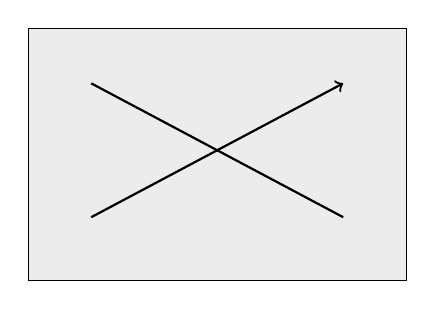
\begin{tikzpicture}
      \draw[fill=gray!15] (0,0) rectangle (4.8,3.2);
      \draw[thick,->] (0.8,0.8) -- (4,2.5);
      \draw[thick] (0.8,2.5) -- (4,0.8);
    \end{tikzpicture}
    \caption{简单示意子图}
    \label{fig:doctor-tikz-sub-left}
  \end{subfigure}
  \hfill
  \begin{subfigure}[b]{0.47\textwidth}
    \centering
    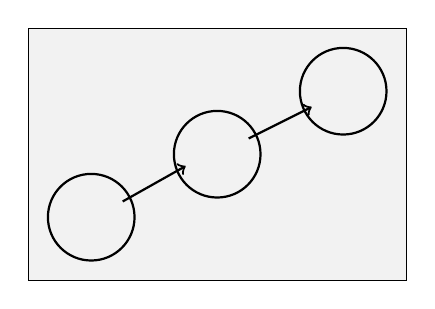
\begin{tikzpicture}
      \draw[fill=gray!10] (0,0) rectangle (4.8,3.2);
      \draw[thick] (0.8,0.8) circle [radius=0.55];
      \draw[thick] (2.4,1.6) circle [radius=0.55];
      \draw[thick] (4.0,2.4) circle [radius=0.55];
      \draw[thick,->] (1.2,1.0) -- (2.0,1.45);
      \draw[thick,->] (2.8,1.8) -- (3.6,2.2);
    \end{tikzpicture}
    \caption{并列对齐子图}
    \label{fig:doctor-tikz-sub-right}
  \end{subfigure}
  \caption{左右两个子图排版示例（TikZ）}
  \label{fig:doctor-tikz-subfigures}
\end{figure}

\cref{fig:doctor-tikz-workflow,fig:doctor-tikz-subfigures} 与上文 \texttt{graphicx} 示例的版式要求一致：图题在图下、子图可对齐引用。

\chapter{表格}\label{ch:doctor-tables}

\section{三线表示例}
\begin{table}[htbp]
  \centering
  \caption{博士示例中常用环境与用途}
  \label{tab:doctor-booktabs}
  \begin{tabular}{lll}
    \toprule
    环境或命令 & 主要用途 & 备注 \\
    \midrule
    \texttt{\textbackslash chapter} & 一级结构组织 & 按章编号 \\
    \texttt{figure} / \texttt{subfigure} & 插图、子图 & 图题置底 \\
    \texttt{table} / \texttt{longtable} & 表格、跨页表 & 表题置顶 \\
    \texttt{equation} / \texttt{align} & 公式 & 可交叉引用 \\
    \texttt{theorem} 等 & 定理类陈述 & 按章编号 \\
    \bottomrule
  \end{tabular}
\end{table}

\section{数值与 \texttt{siunitx}（示意）}
导言区已 \texttt{\textbackslash usepackage\{siunitx\}} 并 \texttt{\textbackslash sisetup\{detect-all\}}，便于物理量与小数列对齐（与本科示例一致）。
\begin{table}[htbp]
  \centering
  \caption{\texttt{siunitx} 的 \texttt{S} 列对齐示例}
  \label{tab:doctor-siunitx}
  \begin{tabular}{S[table-format=3.2] S[table-format=2.1]}
    \toprule
    {\heiti 列甲 / m} & {\heiti 列乙 / s} \\
    \midrule
    12.34 & 1.2 \\
    0.88  & 10.0 \\
    \bottomrule
  \end{tabular}
\end{table}

\section{长表格示例}
\begin{center}
\begin{longtable}{clp{0.52\textwidth}}
  \caption{博士学位论文常见组成部分（示意，以学校最新规范为准）}\\
  \toprule
  序号 & 部分 & 说明 \\
  \midrule
  \endfirsthead
  \caption[]{博士学位论文常见组成部分（续）}\\
  \toprule
  序号 & 部分 & 说明 \\
  \midrule
  \endhead
  \bottomrule
  \endfoot
  1 & 封面与中英文题名页 & 体现题目、作者、导师、专业、研究方向及提交/答辩日期等。 \\
  2 & 独创性声明与版权使用授权书 & 按学校格式签署。 \\
  3 & 目录 & 一般列到二级标题；页码与正文区分编排方式按规范执行。 \\
  4 & 中英文摘要 & 摘要篇幅、关键词数量等按《博士硕士学位论文规范》执行。 \\
  5 & 正文 & 绪论、各章主体、结论等；可分多章展开研究工作。 \\
  6 & 参考文献 & 著录格式与顺序按 GB/T~7714 及学校要求。 \\
  7 & 致谢 & 致谢对象与范围按学校规定。 \\
  8 & 在读期间取得的科研成果 & 已发表论文、专利、会议论文、科研项目等；致谢之后、附录之前。 \\
  9 & 附录 & 补充材料、符号表、程序等，非必须。 \\
\end{longtable}
\end{center}

\chapter{数学公式}\label{ch:doctor-math}

\section{编号与对齐}
\begin{equation}
  J(\boldsymbol{\beta})=\lVert \mathbf{y}-\mathbf{X}\boldsymbol{\beta} \rVert_2^2.
  \label{eq:doctor-objective}
\end{equation}
\begin{align}
  \frac{\partial J}{\partial \boldsymbol{\beta}}
  &= -2\mathbf{X}^{\mathsf T}\left(\mathbf{y}-\mathbf{X}\boldsymbol{\beta}\right)=0, \label{eq:doctor-gradient}\\
  \mathbf{X}^{\mathsf T}\mathbf{X}\boldsymbol{\beta}
  &= \mathbf{X}^{\mathsf T}\mathbf{y}. \label{eq:doctor-normal}
\end{align}
由 \cref{eq:doctor-objective,eq:doctor-gradient,eq:doctor-normal} 可见编号与 \texttt{\textbackslash cref} 引用正常。

\section{常见符号示例}
下列公式展示了常见的集合、极限、求和、积分和矩阵写法：
\begin{equation}
  A=\left\{x\in\mathbb{R}: x^2\le 1\right\}, \qquad
  \lim_{n\to\infty}\sum_{k=1}^{n}\frac{1}{k^2}=\frac{\pi^2}{6}.
\end{equation}
\begin{equation}
  \int_{0}^{1} x^\alpha (1-x)^\beta\,\mathrm{d}x
  = \frac{\Gamma(\alpha+1)\Gamma(\beta+1)}{\Gamma(\alpha+\beta+2)}.
\end{equation}
\begin{equation}
  \mathbf{A}=
  \begin{bmatrix}
    1 & 0 & 2 \\
    0 & 1 & 3 \\
    2 & 3 & 5
  \end{bmatrix}.
\end{equation}

考虑方程组
\begin{equation}\label{eq:doctor-uniform}
\begin{aligned}
  a\cos\theta+b\sin\theta&=10,\\
  b\cos\theta+a\sin\theta&=10
\end{aligned}
  \implies a^2+b^2=100.
\end{equation}
\eqref{eq:doctor-uniform} 演示了 \texttt{aligned} 置于 \texttt{equation} 内的统一编号。

\section{分段函数与方程组}
分段函数可用 \texttt{cases} 环境排版；例如
\[
  f(\theta):=
  \begin{cases}
    a\cos\theta,&\theta\in[\pi,2\pi),\\
    b\sin\theta,&\theta\in[0,\pi).
  \end{cases}
\]

\chapter{定理环境}\label{ch:doctor-theorem}

\section{定理、定义与证明}

\begin{defn}\label{def:doctor-convex}
若对任意 $x,y\in \mathbb{R}^n$ 和任意 $\lambda\in[0,1]$，都有
$f(\lambda x+(1-\lambda)y)\le \lambda f(x)+(1-\lambda)f(y)$，则称 $f$ 为凸函数。
\end{defn}

\begin{thm}[Jensen不等式]\label{thm:doctor-jensen}
设 $f$ 是区间 $I$ 上的凸函数，$x_1,\dots,x_n\in I$，
$\lambda_1,\dots,\lambda_n\ge 0$ 且 $\sum_{i=1}^{n}\lambda_i=1$，则
$f\!\left(\sum_{i=1}^{n}\lambda_i x_i\right)\le \sum_{i=1}^{n}\lambda_i f(x_i)$。
\end{thm}

\begin{proof}
这是 Jensen 不等式的标准表述。对于离散情形，可由凸函数定义反复应用归纳得到。
\end{proof}

\begin{cor}\label{cor:doctor-amgm}
对任意正数 $a_1,\dots,a_n$，有
\[
\frac{a_1+\cdots+a_n}{n}\ge \sqrt[n]{a_1\cdots a_n}.
\]
\end{cor}

\begin{rmk}
在模板中，\texttt{thm}、\texttt{defn}、\texttt{cor} 等缩写环境与全称
（\texttt{theorem}、\texttt{definition}、\texttt{corollary} 等）共享计数器，按章编号，
并可通过 \texttt{\textbackslash cref} 直接引用，如 \cref{def:doctor-convex,thm:doctor-jensen,cor:doctor-amgm}。
\end{rmk}

\chapter{参考文献引用示例}\label{ch:doctor-bib}

\noindent 本示例的 \path{swuthesis-doctor-main.bib} 由主文件内 \texttt{filecontents*} 环境生成；条目著录与公开书目一致，
类型涵盖 GB/T~国标、西文专著、\texttt{CTeX} 手册、中文专著与期刊（可在 CNKI 等检索）、
MathSciNet 著录的数学期刊论文、arXiv 预印本与 NeurIPS 会议论文、学校发布的本科与研究生规范网页等；键名与本科示例 \path{swuthesis-main.bib} 中部分条目对齐，便于对照维护。

\section{正文中的引用}
学术写作中，正文引用应与文后参考文献表一致。使用 \texttt{biblatex} 配合
GB/T~7714 顺序编码样式后，可在正文中混合著录西文专著\cite{knuth1984texbook,lamport1994latex,mittelbach2004companion}、
中文专著（如可在 CNKI 检索的教材）\cite{zhouzhihua2016ml}、中文期刊论文\cite{liguojie2012bigdata}、
英文数学期刊（可在 MathSciNet 按 MR 号或 DOI 核对）\cite{WalpuskiZhang2021DMJ}、
arXiv 预印本\cite{taubes2020compactness}、会议论文\cite{vaswani2017attention}；
排版工具说明见 \cite{ctex2022}，著录格式见国家标准 \cite{gbt7714}；
学校本科与研究生管理文件见 \cite{swu2021thesisManageNotice,swuUndergradThesisSpecWeb,swu2022gradThesisSpecDoc}。

\section{文后文献表}
模板默认提供参考文献章节标题，并将文献表自动加入目录。若继续扩展模板，可在这一层统一控制
文献标题、著录格式以及是否启用 \hologo{biber} 后端。

\backmatter
\printbibliography[heading=bibintoc,title={参考文献}]

\begin{acknowledgements}
行文至此，博士阶段的学习与论文撰写暂告一段落。回首数年，感慨系之。

首谢吾师。先生治学严谨，诲人不倦。自选题立意、文献研读，至方法论证与论文谋篇，皆蒙悉心指点。
每遇疑难，必条分缕析，使吾豁然开朗。师恩厚重，没齿难忘。学海无涯，唯愿日后勤勉，不负师望。

次谢家人。养育之恩、支持之力，非片言可尽。求学之路，赖家庭为后盾，方能专心于学业与研究。

亦谢同窗与师门诸友。或切磋学问，或相勉共进，皆为本论文与本人成长之助。

本示例文档用于展示西南大学博士学位论文模板的主要排版功能：自封面、英文题名页、摘要、目录，
至正文图表、公式、定理、参考文献、致谢、在读期间科研成果及附录，皆依类文件接口组织。
虽为示例，亦力求格式严谨，以资参考。学力所限，疏漏难免，恳请师长斧正。

谨以此文，致谢所有关怀相助之人。

\vspace{\baselineskip}
\begin{flushright}
\begin{tabular}{c}
张三\\
\today\\
于西南大学
\end{tabular}
\end{flushright}
\end{acknowledgements}

\begin{publications}
以下条目为版式示意，正式提交时请按学院要求增删并核对编号、日期与授权号等字段。

\swupublicationsubsection{已发表论文：}
\begin{swupubenum}
  \item 某某. 关于人工智能在学位授予工作中的应用. 人工智能国际研讨会论文集，2023年12月.
  \item 某某. 中国科学技术大学研究生学位论文撰写规范. 中国科学技术大学学报，2024年第1期.
\end{swupubenum}

\swupublicationsubsection{发明专利：}
\begin{swupubenum}
  \item 某某. 一种温热外敷药制备方案. 授权号：CN123456789B，2023-08-12.
  \item （第二条专利条目示意，撰写时替换为真实信息.）
\end{swupubenum}

\swupublicationsubsection{会议论文：}
\begin{swupubenum}
  \item 某某. 关于人工智能在学位授予工作的应用，人工智能国际研讨会，2023年12月.
  \item （第二条会议论文示意.）
\end{swupubenum}

\swupublicationsubsection{参与的科研项目：}
\begin{swupubenum}
  \item 智能计算板卡与整机，科技委重点项目—课题，2018--2020.
  \item （第二条项目示意.）
\end{swupubenum}
\end{publications}

\appendix
\chapter{西南大学本科毕业论文（设计）规范}\label{app:swu-undergrad-spec}

\noindent 为统一本科毕业论文（设计）的撰写和编辑格式，保证本科毕业论文（设计）的质量，便利信息系统的收集加工、检索利用和交流传播，在《西南大学全日制本科学生毕业论文（设计）工作管理办法》（西校〔2021〕4号）基础上，特制定本规范。

\section*{一、基本要求}
\begin{enumerate}
  \item 本科毕业论文（设计）应在导师指导下，由学生本人独立完成，严禁抄袭和剽窃。
  \item 本科毕业论文（设计）应能表明学生确已在本专业学习上掌握了专门知识，并对所研究问题有新的认识或理解，在导师的指导下具备独立解决问题的能力。论文工作时间一般不得少于半年。
  \item 原则上人文社科类专业毕业论文的字数不少于8000字，理工农医类专业毕业论文不少于6000字，艺体类专业毕业论文不少于5000字；毕业论文一般应采用简体中文进行（外语专业、古汉语研究中涉及的古文字和参考文献中引用的外文文献除外）；如学生申请用外语进行书写，需提交申请书，由指导教师同意、系主任和学院（部）主管教学领导审批，且不少于5000个单词；艺术类毕业设计说明书不少于3000字；计算机软件类设计或论文，一般源程序行数不少于2000条，并写出5000字以上的软件说明书或论文。各专业可根据自身特点，在学校基础上提出本专业毕业论文的具体工作量要求。
  \item 凡是不符合上述要求的，一律不接受其毕业论文（设计）答辩申请。
\end{enumerate}

\section*{二、编写格式}
\begin{enumerate}
\item 内容排列编号

毕业论文（设计）内容的顺序编号参照国家标准 GB ``标准章、条、款、项的划分编号和排列格式'' 的有关规定，采用阿拉伯数字分级编号，如：第1章第2条第2款应标为：1.2.2。

\item 论文结构（组成部分与排列顺序）

毕业论文（设计）主要由封面、独创声明与版权使用授权书、目录、中英文作者信息和摘要、导论、正文、结论、参考文献、致谢、附录等部分组成，并按此前后顺序排列。

\begin{enumerate}[label=(\arabic*)]
  \item 封面

  本科毕业论文（设计）采用白色封面。封面格式见附件1。
  \item 独创声明与版权使用授权书

  签署《毕业论文（设计）独创性声明和版权使用授权书》，其格式和内容见附件2。要求每本论文必不可缺，并有亲笔手写体签名。
  \item 目录

  目录包括论文的篇、章、条、款、项、附录等的序号、名称和页码，一般只列到二级标题。目录中文字体采用宋体小四号字，目录中的页码采用Times New Roman，小四号，1.5倍行距。目录本身的页码另编，页码在页下方居中排列，使用罗马数字（Ⅰ、Ⅱ……），编写格式见附件3。
  \item 中英文标题、作者信息、摘要和关键词

  另页置于目录之后，中文排在英文之前，格式见附件4，具体包含以下内容：中文标题、中文作者姓名和单位、中文内容摘要及关键词（中文摘要在300字以内，关键词3--5个）；英文标题、英文作者姓名和单位、英文摘要及关键词（英文摘要以250个实词左右为宜，关键词与中文关键词对应）。
  \item 导论（或引言）

  导论（或引言）可包括问题提出的背景、研究意义、研究目的、研究现状、研究设想、预期结果等。
  \item 正文

  正文是论文的核心部分，可根据内容分成多个章节。由于研究工作涉及的学科领域、研究方法、结果表达方式等有很大的差异，因此，对各学院（部）正文内容的撰写格式不作严格的统一要求，但每个学院内部应保持统一格式。
  \item 结论

  结论是最终的、总体的结论，不是正文中各段的小节的简单重复。结论应该准确、完整、精练。如果不可能导出应有的结论，也可以没有结论而进行必要的讨论。
  \item 参考文献

  参考文献应是论文作者查阅过的对论文具有参考价值的权威性的最新文献。参考文献的列表顺序，采用``著者-出版年制''，中外文文献分开，中文按著者姓氏拼音顺序列出、英文按字母顺序列出，中文排在前，外文排在后，连续编码，并将序号置于方括号中。所有参考文献列于正文末尾，不在各章节后列参考文献。参考文献总数应不少于10篇，其中外文资料至少2篇。
  \item 致谢

  致谢对象限于对完成毕业论文（设计）有较大帮助的单位和个人。
  \item 附录

  附录是作为论文主体的补充项目，如为了论文材料的完整性而补充的一些附加图、表等信息，并不是必须的。
\end{enumerate}
\end{enumerate}
\section*{三、排版要求}
\begin{enumerate}
\item 论文开本及版芯

论文开本大小：210\,mm$\times$297\,mm（A4纸），单面打印。版芯要求：左边距：25\,mm，右边距：25\,mm，上边距：30\,mm，下边距：25\,mm，装订线：10\,mm，页眉边距：23\,mm，页脚边距：18\,mm。

\item 标题：论文分三级标题

一级标题：黑体，四号，居中，段前、段后间距为0.5行；二级标题：黑体，小四号，段前、段后间距为0.5行；三级标题：宋体，小四号，加粗，段前、段后间距为0.5行。

\item 正文字体

正文采用小四号宋体，行间距为1.5倍；正文中的图表应有中英文对照标题，图表编号使用阿拉伯数字分章节排序。图头在图的下方，表头在表格上方，其中中文使用宋体、五号，英文及数字使用Times New Roman、五号。表格采用三线表。

论文中公式使用公式编辑器编写，格式为公式居中，编号右对齐。编号为Times New Roman、小四号。编号使用阿拉伯数字分章节排序。论文中所引用的参考文献需按在正文中出现的顺序以上标进行标注，格式为宋体、小四。

\item 页眉、页脚

除页码之外，不再设其他页眉页脚，页码采用阿拉伯数字形式，居中。

\item 量和单位

严格执行GB3100$\sim$3102：93有关量和单位的规定（参阅《常用量和单位》，计量出版社，1996）。单位名称的书写，可采用国际通用符号，也可用中文名称，但全文应统一。

\item 英文、罗马字符

英文、罗马字符一般采用Times New Roman正体，按规定应采用斜体的采用斜体。
\end{enumerate}
\section*{四、学位论文装袋顺序}
鉴于学生数量较多，由各学院（部）自行决定本单位论文是否统一打印。

装袋顺序：开题报告——教师指导学生毕业论文情况登记表——查重检测报告——指导教师评阅表——交叉评阅表——答辩记录——论文全文——图纸、作品等。

\chapter{Matlab 代码}\label{app:code-matlab}
\zihao{-4}
下面给出一个~Matlab 代码示例。该代码对应
1989年第30届国际数学奥林匹克（IMO）竞赛的一道试题的一种构造思路：\vspace{.5cm}

\noindent 求证：集合$\{1, 2, \ldots, 1989\}$可以分为$117$个互不相交的子集
\[A_i, \qquad i = 1, 2, \ldots, 117\]
使得
\begin{enumerate}[label=\arabic*., leftmargin=2em]
    \item 每个$A_i$都含有$17$个元素；
    \item 每个$A_i$中所有元素之和相同。
\end{enumerate}

代码文件名为~\path{equalsumpartition.m}，运行时在~Matlab 命令窗口输入
\begin{verbatim}
        equalsumpartition(1989,117)
\end{verbatim}
后回车即可。引入代码可使用
\begin{verbatim}
       \lstinputlisting[language=Matlab]{codes/equalsumpartition.m}
\end{verbatim}
注意：文件放在子文件夹~\path{codes/} 时，路径需写为~\path{codes/...}。

\lstinputlisting[language=Matlab]{codes/equalsumpartition.m}

\chapter{Wolfram 语言代码示例}\label{app:code-wolfram}
Wolfram 语言（Wolfram Language）为 Mathematica 所采用的标准名称；\texttt{listings} 宏包仍以
\texttt{language=Mathematica} 作为语法高亮标识，并非笔误。
按当前宏包组合，直接按第~\ref{sec:doctor-code}~节方式引入 \path{.wl} 或笔记本导出代码时，环境配置可能仍需微调。
一种可行做法是将代码另存为 \path{.txt}，再使用
\begin{verbatim}
        \lstinputlisting[language=Mathematica]{myfile.txt}
\end{verbatim}
下面示例文件为~\path{primeSieve.txt}（与旧模板中示例同源），引入命令为
\begin{verbatim}
       \lstinputlisting[language=Mathematica]{codes/primeSieve.txt}
\end{verbatim}
该代码实现 Eratosthenes 筛法：对给定正整数$n$，可求出所有不超过$n$的素数。
示例在$[50,200]$内随机选取$n$（可修改代码中的变量 \texttt{m}、\texttt{M}）；若需查看中间过程，将变量 \texttt{d} 设为非$0$ 即可。
\lstinputlisting[language=Mathematica]{codes/primeSieve.txt}

\chapter{Python 代码}\label{app:code-python}
下面示例与 Wolfram 小节引入方式相同，文件名为~\path{test.txt}（内容对应简单的 \path{test.py} 示例）。
\begin{verbatim}
\lstinputlisting[language=Python]{codes/test.txt}
\end{verbatim}
\lstinputlisting[language=Python]{codes/test.txt}

\chapter{R 代码}\label{app:code-r}
以下示例为寿险精算中分期偿还利息与本金划分的简单演示（与旧模板示例同源），文件名为~\path{example.R}，在 \textbf{R} 中打开运行即可。
\begin{verbatim}
       \lstinputlisting[language=R]{codes/example.R}
\end{verbatim}
\lstinputlisting[language=R]{codes/example.R}

\chapter{DES 的 C++ 代码}\label{app:code-cpp}
下面示例文件为~\path{mytestdes.cpp}，实现对称密码算法~DES。
\begin{verbatim}
       \lstinputlisting[language={[ANSI]C++}]{codes/mytestdes.cpp}
\end{verbatim}
\lstinputlisting[language={[ANSI]C++}]{codes/mytestdes.cpp}

\chapter*{附录示例来源说明}
\phantomsection\label{app:source-note}
下列程序附录的例题与源码文件改编自包小敏老师长期维护的西南大学本科毕业论文\LaTeX{}模板\cite{bao2024swuthesisLegacy}（坊间常称「本科毕业论文模板\_新」等），原模板面向数学与统计学院本科毕业论文，版心尺寸按学校要求设置；其首版可追溯至 2006 年，经多年修订，近年已随学校格式调整与 \hologo{XeLaTeX} 编译方式更新。

本仓库 \texttt{swuthesis} 并非在该模板源码上直接修改，而是全新类文件与主文档结构；此处仅保留经典代码示例，便于对照 \texttt{listings} 用法。
首次使用请先阅读\cref{ch:doctor-guide}；公式环境见\cref{ch:doctor-math}，定理类环境见\cref{ch:doctor-theorem}；插图与表格分别见\cref{ch:doctor-figures}、\cref{ch:doctor-tables}；参考文献著录示例见\cref{ch:doctor-bib}；程序代码引入方式见\cref{sec:doctor-code}，各语言完整示例见附录\ref{app:code-matlab}--\ref{app:code-cpp}。

\end{document}
%</doctor>
%    \end{macrocode}

%
% \Finale
